\chapter{REGULARIZATION METHODS FOR SUBSET ARMA SELECTION}
\label{chap:co2}

\section{Introduction}

Let $\{y_t: t=1,2,\cdots,T\}$ be a sequentially observed discrete and equally-spaced sample from a weakly stationary, homoskedastic process $\{Y_t:t=\cdots,-1,0,1,\cdots\}$. For the purpose of forecasting future realizations i.e. $\hat{y}_{T+h}$ where $h\in\mathbb{N}$, a model of the general form $$y_{t}=f(y_{t-1},y_{t-2},\cdots,y_{t-p},\epsilon_{t-1},\epsilon_{t-2},\cdots,\epsilon_{t-q})+\epsilon_t$$ is used. Under homoskedasticity, $\{\epsilon_t\}$ is assumed to be white noise with mean 0 and variance $\sigma^2$.  Finite order parameters $p,q\in\mathbb{N}$ quantify the strength that past information has on prediction. Define $m=\max\{p,q\}$. In most cases, $m$ is small relative to $T$; however, when cyclical phenomenon is detected, $m\geq s$ where $s$ is the seasonal periodicity. The latter scenario leads to long gaps in relevant information for forecasting.

The seasonal autoregressive moving average (SARMA) process, popularized by \cite{Box1976}, jointly models the temporal short-term and seasonal dynamics of $\{y_t\}$ to forecast future unknown realizations. Let $B$ represent the backshift operator  where $B^ky_{t}=y_{t-k}$ and define polynomial functions $\Phi(B^s)=1-\sum\limits_{J=1}^P \Phi_J B^{sJ}$, $\phi(B)=1-\sum\limits_{j=1}^p \phi_j B^{j}$, $\Theta(B^s)=1+\sum\limits_{K=1}^Q \Theta_K B^{sK}$, and $\theta(B)=1+\sum\limits_{k=1}^q \theta_k B^{K}$. If the seasonal periodicity $s>1$ is known, the SARMA$(p,q)\times(P,Q)_{s}$ process in Equation \ref{eq:sarma} represents a viable family of models for forecasting.
\begin{equation}
\label{eq:sarma}
\Phi(B^s)\phi(B)y_t=\Theta(B^s)\theta(B)\epsilon_t
\end{equation}

The seasonal periodicity $s$ is typically unknown \textit{a priori}. Any SARMA model from Equation \ref{eq:sarma} algebraically reduces to an ARMA$(p^*,q^*)$ process $\phi^*(B)y_t=\theta^*(B)\epsilon_t$ where $\max\{p^*,q^*\}=\max\{Ps+p,Qs+q\} \textrm{ where } [p,P,q,Q,s]'\in\mathbbm{N}^5$. For example, consider a quarterly SARMA$(1,0)\times(1,0)_{4}$ process $\{x_t\}$ where $\phi_1=0.6$ and $\Phi_1=0.3$. The temporal dynamics of $\{x_t\}$ are equivalently modeled using an ARMA$(5,0)$ process such that $\bm{\phi}=[\phi_1,\phi_2,\phi_3,\phi_4,\phi_5]'=[0.6,0,0,0.3,-0.18]'$ (see Equation \ref{eq:sarma2arma}).
\begin{equation}
\label{eq:sarma2arma}
\begin{split}
\Phi(B^4)\phi(B)x_t&=\epsilon_t\\
(1-0.3B^4)(1-0.6B)x_t&=\epsilon_t\\
(1-0.6B-0.3B^4+0.18B^5)x_t&=\epsilon_t\\
\end{split}
\end{equation}

Fitting an ARMA$(p^*,q^*)$ model to an arbitrary series $\{y_t\}$ requires estimation of AR coefficients $\bm{\phi}=[\phi_1,\cdots,\phi_{p*}]'$ and MA coefficients $\bm{\theta}=[\theta_1,\cdots,\theta_{q^*}]'$. Estimates $\hat{\bm{\phi} }$ and $\hat{\bm{\theta} }$ that validate stationary and invertible regulatory assumptions are desired. Stationarity and invertibility require all roots of both characteristic equations, $1-\phi_1z-\phi_2z^2-\cdots -\phi_{p^*}z^{p^*}=0$ and $1+\theta_1z+\theta_2z^2+\cdots +\theta_{q^*}z^{q^*}=0$, to be outside the unit circle. Classically, parameter estimation is conducted via method of moments, least squares, or maximum likelihood \citep{Hamilton1994, Cryer2008}. When $q^*=0$, these approaches are simple extensions of linear regression where the set of predictor variables are lagged realizations of the time series. If $q^*>0$, a linear model representation exists, but the presence of MA terms poses an estimation problem since the innovations $\{\epsilon_t\}$ are unobservable and dependent on $\bm{\phi}$ and $\bm{\theta}$. Popular least squares and maximum likelihood estimation methods become far less efficient and require nonlinear optimization techniques.

Any ARMA$(p^*,q^*)$ model that satisfies the invertibility condition has an $AR(\infty)$ representation, i.e. $(1-\sum\limits_{j=1}^\infty \phi^\prime_jB^j)y_t=\epsilon_t$. If $\bm{\phi}^\prime$ is known, the full set of $\{\epsilon_t\}$ can be obtained. The residuals $\{\hat{\epsilon}_t: t=p^\prime+1,\cdots,T\}$ of a long AR$(p^\prime)$ process fitted to  $\{y_t\}$ can approximate the unobserved $\{\epsilon_t\}$.  This approach was initially proposed by \cite{Hannan1982} to obtain quick estimation of ARMA$(p^*,q^*)$ as it avoids previously mentioned estimation issues. For further information, see \citet[pp. 156-158]{Brockwell2016}.

The model orders $p^*$ and $q^*$ can be heuristically selected through inspection of sample autocorrelation and partial autocorrelation functions (abbreviated ACF and PACF, respectively). This non-scientific approach could lead to misspecified models and possibly poor forecasting performance. Suppose $p$ and $q$ are safe upper bounds such that $p\geq p^*$ and $q\geq q^*$. For the $pq$ different ARMA models, final order selection can be based off minimization of some measure of prediction error (PE). Information criteria such as AIC \citep{Akaike1974} or BIC \citep{Schwarz1978} are popular metrics that penalize for model complexity. Stepwise selection algorithms are usually instituted to accelerate this process.

These approaches are best suited for estimating ARMA processes where $\phi_j\neq 0$ and $\theta_k \neq 0$ for $j\in\{1,\cdots,p^*\}$ and $k\in\{1,\cdots,q^*\}$. For the scenario in Equation \ref{eq:sarma2arma}, correct identification of $p^*=5$ and $q^*=0$ still leads to overfitting since truly zero parameters, $\phi_2$ and $\phi_3$, are included in estimation. The true process in Equation \ref{eq:sarma2arma} is a a subset ARMA$(5,0)$ model where $\bm{\phi}=[\phi_1,\phi_4,\phi_5]'=[0.6,0.3,-0.18]'$. Common approaches for ARMA$(p,q)$ model selection become less efficient and reliable when searching through the $2^{(p+q)}$ unique subset ARMA$(p,q)$ models.	

Let $\bm{y}=[y_{m},\cdots,y_T]'$, $\bm{\epsilon}=[\epsilon_{m},\cdots,\epsilon_T]'$, $\bm{\beta}=[\bm{\phi}',\bm{\theta}']'=[\phi_1,\cdots,\phi_p,\theta_1,\cdots,\theta_q]'$, and 
\begin{equation*}
\bm{X}=\begin{bmatrix} \bm{x}'_{m}  \\
					\bm{x}'_{m+1}  \\
					\vdots \\
					\bm{x}'_{T} \\
	\end{bmatrix} =
	\begin{bmatrix} y_{m-1} & \cdots & y_{m-p} &
					\hat{\epsilon}_{m-1} & \cdots & \hat{\epsilon}_{m-q} \\
					y_{m} & \cdots & y_{m-p+1} &
					\hat{\epsilon}_{m} & \cdots & \hat{\epsilon}_{m-q+1} \\
					\vdots & \ddots & \vdots &\
					\vdots & \ddots & \vdots & \\
					y_{T-1} & \cdots & y_{T-p} &
					\hat{\epsilon}_{T-1} & \cdots & \hat{\epsilon}_{T-q} \\
	\end{bmatrix}.
\end{equation*}
The ARMA$(p,q)$ model is equivalently represented by $\bm{y}=\bm{X}\bm{\beta}+\bm{\epsilon}$. Recall that $\hat{\epsilon}_t$ are residuals from fitted AR$(p^\prime)$ models used to estimate unknown innovations. Similar to estimation via conditional least squares and conditional maximum likelihood \citep{Hamilton1994}, the first $m-1$ observations are lost in parameter estimation where $m=p^\prime+max\{p,q\}+1$. For reduction of $m$, selection of $p^\prime$ can be based off AIC or BIC  \citep{Hannan1984a,Chen2011}. Also, it is important to note $\{y_t\}$ is assumed to be mean-centered. An additional mean parameter $\mu$ can be included in $\bm{\beta}$ via  binding a column of $1$s to $\bm{X}$.

Presenting the ARMA$(p,q)$ model as a linear Gaussian model is quite advantageous. For both linear and generalized linear models, the least absolute shrinkage and selection operator (LASSO) of \cite{Tibshirani1996} efficiently combines model selection and estimation. The LASSO estimator in Equation \ref{eq:lasso2} achieves sparsity through $\ell_1$ penalization of the least squares criterion.  The tuning parameter $\lambda >0$ controls overall shrinkage of $\bm{\beta}$ towards 0. Consequentially, the LASSO estimate is a function of $\lambda$, but full solution paths are quickly obtained via well-developed algorithms \citep{Efron2004}. The optimal $\lambda$ is often based off minimization of AIC, BIC, or some generalization of prediction error. The effectiveness of LASSO motivated analogous Bayesian approaches using Laplace priors \citep{Park2008, Yuan2005}. Similarly, hyperpriors placed on $\lambda$ encourage data-driven shrinkage of posterior estimates.
\begin{equation}
\label{eq:lasso2}
\hat{\bm{\beta}}_{L} (\lambda)= \underset{\bm{\beta}}{\textrm{argmin }}  ||\bm{y}-\bm{X}\bm{\beta}||^2 + \lambda \sum\limits_{i=1}^{p+q}|\beta_i|
\end{equation}

Applying LASSO in time series analysis is potentially problematic since the ARMA model matrix $\bm{X}$ contains correlated predictors.  \cite{Nardi2011} explored the consistency properties of $\hat{\bm{\beta}}_{L}$ for AR$(p)$ processes to approximate realizations from ARMA data generating processes (DGPs). However, high correlation between non-zero and irrelevant ARMA predictors may violate the ``irrepresentable condition" required for sign and model selection consistency \citep{Zhao2006}. \cite{Hebiri2013} demonstrate that highly collinear designs yield underestimation of $\lambda$ and poor prediction. Modified LASSO and other methods with better asymptotic properties mitigate the consequences of correlated predictors.

In this context, $p$ and $q$ should be safely overestimated, resulting in a sparse parameter vector $\bm{\beta}$. In this article, the application of regularization methods to automate subset ARMA$(p,q)$ selection and estimation of $\bm{\beta}$ is explored. Section \ref{sec:methods} presents three different methods that incorporate subset selection through regularization estimation. The first two methods extend off work from \cite{Chen2011}. A discussion of cross-validation techniques explores alternative ways to select regularization tuning parameters. The final regularization method is developed under the Bayesian framework for a contrast to the preceding classical approaches. Section \ref{sec:mc} contains simulation studies evaluating and comparing the different methods. Section \ref{sec:co2app} applies the methods to monthly carbon dioxide time series collected from two atmospheric observatories.










\section{Methods}
\label{sec:methods}

Assume $y_t$ follows a subset ARMA$(p,q)$ process. Recall the matrix ARMA representation $\bm{y}=\bm{X}\bm{\beta}+\bm{\epsilon}$ where $\bm{\beta}=[\bm{\phi}',\bm{\theta}']=[\beta_1,\cdots,\beta_{p+q}]'$. The set $\mathcal{V}=\{i:\beta_i\neq 0\}$ indicates the AR and MA terms relevant to the true process. If the cardinality $|\mathcal{V}|<p+q$, irrelevant predictors are included in the ARMA model matrix $\bm{X}$. Given observed data $\{y_t: t=m,m+1,\cdots,T\}$, $\hat{\bm{\beta}}$ is an estimator for $\bm{\beta}$ and $\hat{\mathcal{V}}=\{i:\hat{\beta}_i\neq 0\}$ for $\mathcal{V}$. Multiple researchers have theoretically explored the asymptotic behavior of penalized estimators including the popular oracle property \citep{Fan2001,Fan2004,Fan2011}. A method for estimating $\bm{\beta}$ is described as oracle if the estimator $\hat{\bm{\beta}}$ asymptotically behaves as an estimator developed under prior knowledge of $\mathcal{V}$. Under these considerations, outlined approaches estimate ARMA coefficients while simultaneously identifying $\mathcal{V}$ through shrinking irrelevant effects to 0.

\subsection{Adaptive LASSO}

\cite{Zou2006} highlighted the conditional consistency of LASSO and introduced adaptive LASSO (ADLASSO) which enjoys the oracle properties. For a chosen $\eta>0$, define the vector of weights $\hat{\bm{w}}=|\hat{\bm{\beta}}+1/T|^{-\eta}$ where $\hat{\bm{\beta}}$ represents an initial estimate of $\bm{\beta}$ derived using ordinary least squares (OLS), ridge, or LASSO regression. The additional $1/T$ exists so division by $0$ is prevented. The ADLASSO estimator $\hat{\bm{\beta}}_{AL}$ is described in Equation \ref{eq:adlasso2}. The tuning parameter $\lambda>0$ controls the degree of penalization across all ARMA terms while coefficient-specific weights fine tune shrinkage.
\begin{equation}
\label{eq:adlasso2}
\hat{\bm{\beta}}_{AL} (\lambda)= \underset{\bm{\beta}}{\textrm{argmin }}  ||\bm{y}-\bm{X}\bm{\beta}||^2 + \lambda \sum\limits_{i=1}^{p+q} \hat{w}_{i}|\beta_i|
\end{equation}

For subset ARMA model selection, \cite{Chen2011} showed ADLASSO is an oracle procedure under 3 regulatory assumptions when $\hat{\bm{\beta}}=(\bm{X}'\bm{X})^{-1}\bm{X}'\bm{y}$. Proof of this result followed from using a long AR$(p^\prime)$ process to estimate unknown innovations. Simulation results indicated best empirical performance when the initial estimate $\hat{\bm{\beta}}=\hat{\bm{\beta}}_L$. Following from \cite{Zou2006} and \cite{Chen2011}, $\eta=2$ and $\hat{\bm{\beta}}_L$ is used for the formulation of $\hat{\bm{w}}$.

\subsection{Adaptive Elastic Net}
The ADLASSO procedure has become popular in time series analysis since parsimonious models typically improve forecasting. Incorporating lags of exogenous time series in $\bm{X}$ adds complexity that ADLASSO can discriminate against. Assuming information becomes less relevant for forecasting as time passes has encouraged modifications for more complicated full models. For example, lag lengths can be included in the functional representation of $\hat{\bm{w}}$ to further encourage penalization for long-lagged terms \citep{Park2013,Konzen2016}. When seasonal effects are prevalent, these ADLASSO modifications may completely eliminate important terms at long lags. 

The elastic net (ENET) of \cite{Zou2005} has applicability in this context where $\bm{X}$ contains two groups of predictors with potentially high pairwise collinearity. Although variable selection benefits of LASSO would be lost, the ridge estimator of \cite{Hoerl1970} could lead to better forecasting. The ENET estimator in Equation \ref{eq:enet}  introduces another tuning parameter $\alpha\in[0,1]$ to influence the trade-off between $\ell_1$ and $\ell_2$ penalties \citep{DeMol2009}. The original motivation of ENET was to overcome model selection limitations of LASSO when the number of parameters is larger than the sample size, a common problem in bioinformatic data \citep{Zou2005}. This problem is not prevalent in time series analysis; however, seasonal dynamics, which require multiple cycles to estimate, are difficult to identify when data is limited and/or the period is large. Hypothetically, it makes sense to evaluate empirical performance of ENET in this context.
\begin{equation}
\label{eq:enet}
\hat{\bm{\beta}}_{E} (\lambda,\alpha)= \underset{\bm{\beta}}{\textrm{argmin }}  ||\bm{y}-\bm{X}\bm{\beta}||^2 + \lambda\bigg[ (1-\alpha) \sum\limits_{i=1}^{p+q} \beta^2_i+ \alpha\sum\limits_{i=1}^{p+q} |\beta_i| \bigg]
\end{equation}

As previously seen, ADLASSO satisfies the oracle properties \citep{Zou2006} and ENET \citep{Zou2005} manages collinearity. \cite{Zou2009a} exploit both advantages by modifying the $\ell_1$ penalty Equation \ref{eq:enet} to match the weighted form in Equation \ref{eq:adlasso2}. This adaptive ENET (ADENET) estimator is formally presented in Equation \ref{eq:aenet}. \cite{Zou2009a} recommend selecting $\hat{\bm{\beta}}=\hat{\bm{\beta}}_{E}$. Since $\hat{\bm{\beta}}_{E}$ depends on the choice of two tuning parameters, $\lambda$ and $\alpha$, optimal selection requires a grid search. Upon empirical evaluation, setting $\hat{\bm{\beta}}=\hat{\bm{\beta}}_{L}$ is sufficient for obtaining the initial weights.
\begin{equation}
\label{eq:aenet}
\hat{\bm{\beta}}_{AE} (\lambda,\alpha)= \underset{\bm{\beta}}{\textrm{argmin }}  ||\bm{y}-\bm{X}\bm{\beta}||^2 + \lambda\bigg[ (1-\alpha)  \sum\limits_{i=1}^{p+q} \beta^2_i+ \alpha\sum\limits_{i=1}^{p+q} \hat{w}_{i}|\beta_i| \bigg]
\end{equation}


\subsection{Options for Selecting Tuning Parameters}
The adaptive estimators $\hat{\bm{\beta}}_{AL} (\lambda)$ and $\hat{\bm{\beta}}_{AE} (\lambda,\alpha)$ depend on choices for $\lambda$ and $\alpha$. Given finite sets $\mathcal{L}=\{\lambda_j>0: j=1,\cdots,J\}$ and $\mathcal{A}=\{0<\alpha_k<1: k=1,\cdots,K\}$, full solution paths for both estimators can be produced via LARS algorithm \citep{Efron2004} or coordinate descent \citep{glmnet}. Essentially, each $\lambda\in\mathcal{L}$ and $\alpha\in\mathcal{A}$ corresponds to a different subset ARMA$(p,q)$ model, equating to $|\mathcal{L}|$ different ADLASSO models and $|\mathcal{L}|\times|\mathcal{A}|$ different ADENET models. The optimal $\lambda^*$ and $\alpha^*$ should be empirically chosen based off some estimate of forecasting performance. In this section, different algorithms to select final subset ARMA models, $\hat{\bm{\beta}}_{AL}=\hat{\bm{\beta}}_{AL}(\lambda^*)$ and $\hat{\bm{\beta}}_{AE}=\hat{\bm{\beta}}_{AE}(\lambda^*,\alpha^*)$, are explained. See \citet[pp. 241-254]{Hastie2009a} for classic approaches to select tuning parameters.

\subsubsection{SELECTION BASED ON AIC OR BIC}

Popular information criteria AIC and BIC can be used to select tuning parameters $\lambda$ and $\alpha$. These penalized measures of error effect model selection for the initial LASSO-based weights $\hat{\bm{w}}$ and final models. To quantify model complexity, consider the approximate degrees of freedom $\hat{v}(\lambda)$=$|\widehat{\mathcal{V}}(\lambda)|$ where $\widehat{\mathcal{V}}(\lambda)=\{i:\hat{\beta}_i\neq 0\}$ \citep{Zou2007}. The AIC and BIC formulas for LASSO and ADLASSO are given in Equation \ref{eq:aicbic}. For ENET and ADENET, $\hat{\bm{\beta}}(\lambda)$ and $\hat{v}(\lambda)$ must be replaced with $\hat{\bm{\beta}}(\lambda,\alpha)$ and $\hat{v}(\lambda,\alpha)$.
\begin{equation}
\label{eq:aicbic}
\begin{split}
\textrm{AIC}(\hat{\bm{\beta}}(\lambda))&=2\hat{v}(\lambda)+(T-m+1)\log\bigg(\frac{||\bm{y}-\bm{X}\hat{\bm{\beta}}(\lambda)||^2}{T-m+1}\bigg)\\
\textrm{BIC}(\hat{\bm{\beta}}(\lambda))&=\log(T-m+1)\hat{v}(\lambda)+(T-m+1)\log\bigg(\frac{||\bm{y}-\bm{X}\hat{\bm{\beta}}(\lambda)||^2}{T-m+1}\bigg)\\
\end{split}
\end{equation}

Choice of information criteria (BIC or AIC) is not a Bayesian versus non-Bayesian argument, but an argument about whether true models exist and can be discovered \citep{burnham2003}. Empirical analysis indicates AIC more frequently outperforms in prediction, but BIC's stronger penalty notoriously leads to better model selection \citep{Burnham2004}. The true complexity of the unknown DGP and the path of AIC/BIC influence this decision\citep{Shao1997,burnham2003}. \cite{Chen2011} consider AIC and BIC in both stages of ADLASSO and acknowledge this phenomenon in simulation of subset ARMA models.  Averaged models weighted based off AIC and BIC are often superior in prediction to individual models, but this is out of the scope of this paper \citep{Burnham2004}. 

Philosophical differences aside, both measures are utilized in model selection and forecasting. ADLASSO and ADENET are two stage procedures. In \cite{Chen2011}, only BIC is used for LASSO estimated weights. These weights are crucial in the overall effectiveness of both estimation algorithm. If the BIC penalty overshrinks estimates toward $0$, relevant parameters can be unrecognized in the second stage regardless of whether AIC or BIC are used. AIC is favored in the first stage providing safer protection against losing too many key variables. To provide comparison to \cite{Chen2011}, consider the three of four possible combinations: AIC in both stages, AIC then BIC, and BIC in both stages. The third option was evaluated in \cite{Chen2011}.

\subsubsection{Selection Based on Cross-Validation}

Optimal tuning parameters for regularization are typically chosen via cross-validation (CV) \citep{Hastie2009a}. This approach has been popular for model selection in classic linear regression since \cite{Stone1974}. For $K$-Fold CV (CV-K), begin by splitting the usable $T-m+1$ portion of the time series into $K$ separate folds. Each fold acts as a testing period for models fitted to remaining data. Figure \ref{fig:kcvplots} illustrates this partitioning for CV-5 and CV-10 assuming $T-m+1=100$. Random assignment of data to $K$ folds leads to approximately $100/K$ prediction points in each data split.
\begin{figure}[htbp!]
	\caption{General $K$-fold Cross-Validation for Model Selection for $K=5$ (top) and $K=10$ (bottom)}
	\center
	\label{fig:kcvplots}
	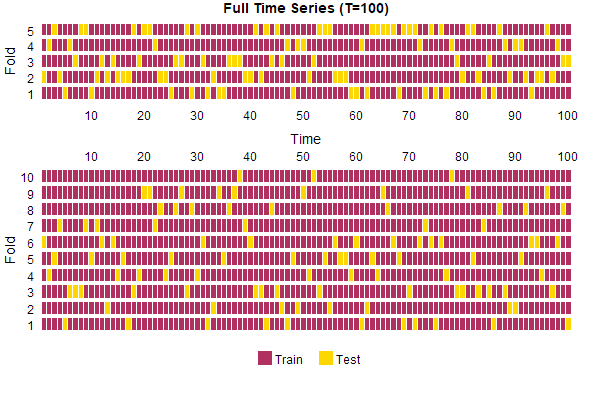
\includegraphics[scale=0.58]{kcvplots}
\end{figure}

Following similar notation from \cite{Hastie2009a}, $\kappa:\{m,m+1,\cdots,T\}\to\{1,\cdots,K\}$ is the indexing function mapping data to specific testing groups. An estimate of PE is obtained for each $\lambda \in \mathcal{L}$ and $\alpha \in \mathcal{A}$, and optimal tuning parameters are chosen based on minimization of this estimate. Specifically for the LASSO cases, $\widehat{\textrm{PE}}(\lambda)$ is expressed in Equation \ref{eq:lassocvpe}. Use $\hat{\bm{\beta}}_{\kappa(t)}(\lambda)$ to represent the estimated ARMA parameters from models fitted to data not in the $\kappa(t)$ group. The most exhaustive case is leave-one-out CV (LOOCV) where $K=(T-m+1)$ and  $\kappa(t)=t-m+1$. Obtaining $\widehat{\textrm{PE}}(\lambda)$ for LOOCV would be time consuming if not for the generalized CV (GCV) of \cite{Wahba1978}.
\begin{equation}
\label{eq:lassocvpe}
	\widehat{\textrm{PE}}(\lambda)=\frac{1}{T-m+1}\sum\limits_{t=m}^T \bigg(y_t-\bm{x}_t'\hat{\bm{\beta}}_{\kappa(t)}(\lambda)\bigg)^2
\end{equation}


\subsubsection{Selection Based on Out-of-Sample Evaluation}

Applied statisticians prefer CV-K or LOOCV when data is cross-sectional. This approach is not intuitive for time series data where prediction on a randomly selected subset of the full data does not seem like forecasting. For a particular $\tau\in (0,1)$, the out-of-sample (OOS) method estimates $\hat{\bm{\beta}}(\lambda)$ from the first $(1-\tau)\times 100\%$ of the data (TRAIN) and forecasts on the final $\tau\times 100\%$ (TEST). Equation 
\ref{eq:lassooos} equates to mean squared forecast error (MSFE) and is used to optimally select tuning parameters. 
\begin{equation}
\label{eq:lassooos}
	\widehat{\textrm{PE}}(\lambda)=\frac{1}{\tau T}\sum\limits_{t\in \textrm{TEST}} \bigg(y_t-\bm{x}_t'\hat{\bm{\beta}}(\lambda)\bigg)^2
\end{equation}

For subset ARMA selection, order parameters $p$ and $q$ are fixed and quantify the memory required to forecast.  In this naive description of OOS, the fact, that some of the forecasts in the TEST period are obtained using data in the TRAIN period, is ignored. Given $p$ and $q$, the final $d=\max\{p,q\}$ points in the TRAIN period are neglected in model fitting. Now, models are strictly evaluated on future data independent of the TRAIN period. In some literature, this is default OOS \citep{Bergmeir2018}; however, this modified version, abbreviated depOOS, highlights the additional considerations being made. Figure \ref{fig:oosplots} displays the difference data division between OOS and depOOS.

\begin{figure}[htbp!]
	\caption{Variations of Out-of-Sample Procedures for Model Selection}
	\center
	\label{fig:oosplots}
	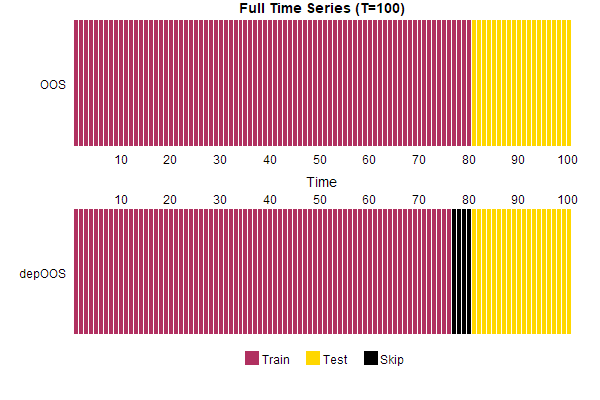
\includegraphics[scale=0.58]{oosplots}
\end{figure}


\subsubsection{Selection Based on Blocked CV}
Classic CV estimates the expected PE constructed from predictions on unfitted data. This may lead to a poor estimate for time series data where the popular ``independent observation" assumption is violated \citep{Arlot2010}. \cite{Burman1994} modified LOOCV by ignoring the $d$ observations before and after each time point in fitting. Similarly, \cite{Bergmeir2018} describe and evaluate a non-dependent version CV-K. For $T-m+1=100$ and $d=4$, this modification, illustrated in Figure \ref{fig:depkcvplots}, is based off the same random assignment in Figure \ref{fig:oosplots}. Controlling the number of points available for fitting models is difficult for this modified CV-K even for a low order $d$. This along with the poor empirical results in \cite{Bergmeir2018} removes this approach from consideration.

\begin{figure}[htbp!]
	\caption{Non-Dependent $K$-fold Cross-Validation for Model Selection for $K=5$ (top) and $K=10$ (bottom)}
	\center
	\label{fig:depkcvplots}
	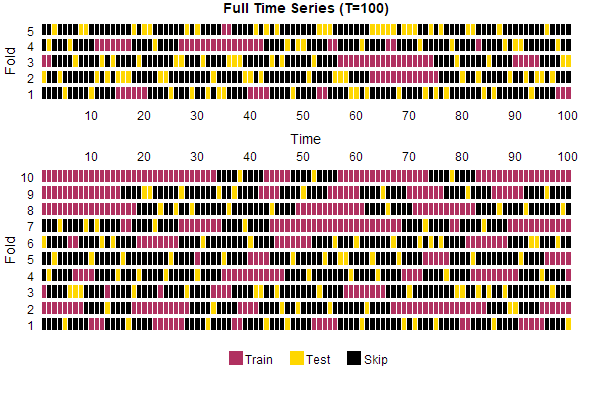
\includegraphics[scale=0.58]{depkcvplots}
\end{figure}

In this paper, blocked variants of CV retain the ordered structure and ensure reasonable sample sizes for model fitting. \cite{Racine2000} alters the CV method of \cite{Burman1994} to measure prediction error on blocks of data around each data point for each fold. \cite{Bergmeir2012} proposes K-fold blocked CV (BCV-K) where naturally ordered data is evenly split into $K$ sets.  For order $d$, the first and last $\lceil \frac{d}{2} \rceil$ data points are removed from each block to remove dependence, and ordinary CV is performed using the blocks. See Figure \ref{fig:bcvplots} for for BCV-5 and BCV-10 when $d=4$. 

\begin{figure}[htbp!]
	\caption{Non-Dependent $K$-Block Cross-Validation for Model Selection for $K=5$ (top) and $K=10$ (bottom)}
	\center
	\label{fig:bcvplots}
	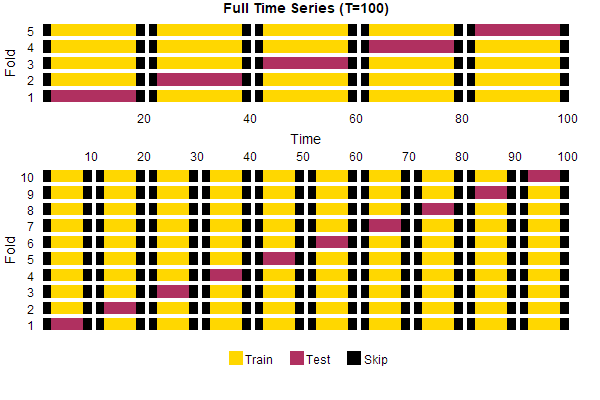
\includegraphics[scale=0.58]{bcvplots}
\end{figure}

Analogous to LOOCV, leave-one-block-out design (LOBOCV) is a natural extension of BCV-K. This approach is similar to $\textrm{BCV-K}^*$ when $K^*=\lfloor \frac{T-m+1}{d} \rfloor$ since the time series is sequentially divided into $K^*$ blocks. Block specific estimates $\widehat{\textrm{PE}}_K(\lambda)$ or $\widehat{\textrm{PE}}_K(\lambda,\alpha)$ are evaluated after models are fitted to data in non-adjacent blocks. In LASSO cases, overall BCV prediction error is based on expression in Equation \ref{eq:lobocv2}. Similar expressions are seen for BCV-5 and BCV-10 since all prediction periods are of the same length. This is a key difference to the initial proposed non-dependent CV-K.
\begin{equation}
\label{eq:lobocv2}
	\widehat{\textrm{PE}}(\lambda)=\frac{1}{K}\sum\limits_{k=1}^K \widehat{\textrm{PE}}_K(\lambda)
\end{equation}

\begin{figure}[htbp!]
	\caption{Leave-One-Block-Out Cross-Validation for Model Selection}
	\center
	\label{fig:lobocvplots}
	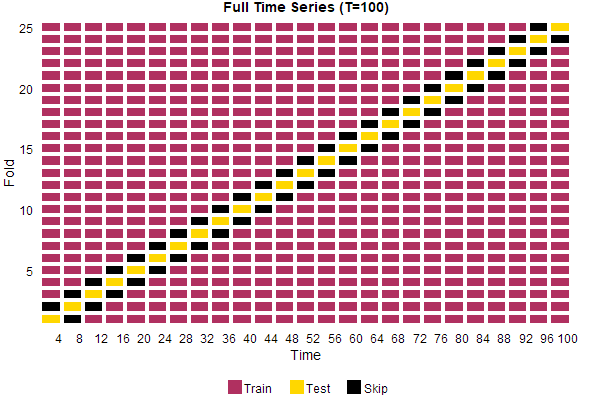
\includegraphics[scale=0.58]{lobocvplots}
\end{figure}

Literature evaluates these methods on the error between estimated $\widehat{\textrm{PE}}$ using CV and OOS and true $\textrm{PE}$ from data completely ignored \citep{Bergmeir2014,Bergmeir2018}. Typical experiments examine this error when the fitted models are known to be misspecified \citep{Burman1994,Racine2000,Bergmeir2018}. These discussions are not the focus of this paper. Only the performance of these methods in selection of $\lambda$ and $\alpha$ for ADLASSO and ADENET is evaluated. 

\subsection{Bayesian Predictive Posterior Projection Method}
\subsubsection{Traditional Bayesian Model Selection}
Classic Bayesian model selection starts by reparamaterizing $\beta_i^*=\xi_i\beta_i$ where $\xi_i\in\{0,1\}$. For the new vector of parameters $\bm{\beta}^*=[\beta^*_1,\beta^*_2,\cdots,\beta^*_{p+q}]'$, the set of relevant parameters $\mathcal{V}=\{i:\beta^*_i\neq 0\}=\{i:\xi_i\neq 0\}$. Let $\mathcal{N}_p(\bm{\mu},\sigma^2\bm{\Sigma}_p)$ represent the $p$-dimensional multivariate normal distribution and $BERN(\pi)$ represent the $Bernouilli$ distribution. If dimension $p$ is not given, assume $p=1$. The scenario $\bm{\Sigma}_p=\bm{I}_p$, where $\bm{I}_p$ is $p\times p$ identity matrix, implies that $\beta_j\perp\beta_k$ for all $j\neq k$. For the new linear model  $\bm{y}=\bm{X}\bm{\beta}^*$, \cite{Kuo1998} suggested the prior $p(\beta_i,\xi_i)=p(\beta_i)p(\xi_i)$ indicating $\beta_i \perp \xi_i$. Later authors suggested $p(\beta_i,\xi_i)=p(\beta_i|\xi_i)p(\xi_i)$ where $p(\beta_i|\xi_i)=(1-\xi_i)p(\beta_i|\xi_i=1)+\xi_i p(\beta_i|\xi_i=0) $ is a mixture prior \citep{Carlin1995}. The popular ``spike and slab" prior is of this type where the slab $p(\beta_i|\xi_i=1)$ is uninformative and the spike $p(\beta_i|\xi_i=0)$ is concentrated around 0 \citep{Mitchell1988,George1993, Carlin1995}. Common to all methods, $\xi_i \sim BERN(\pi_{i,0})$ where $\pi_{i,0}$ is the prior probability that variable $\beta_i \neq 0$. All subset models are equally likely \textit{a priori} when $\pi_{i,0}=0.5$. Sampling from $p(\bm{\beta},\bm{\xi},\sigma^2|\bm{y},\bm{X})$ requires a combination of approaches \citep{Dellaportas2002}, and the posterior mode of $\bm{\xi}$ indicates the best model. Posterior model probabilities and Bayes factors are used to discriminate between possible sub models. Implementation of Bayesian model averaging is within this umbrella \citep{Raftery1997,Hoeting1998,Hoeting1999}.

\subsubsection{Bayesian Regularization}
Posterior samplers based on 2-component mixture priors are often slow in exploring high-dimensional spaces. Priors developed from continuous mixing densities achieve similar results without requiring tuning. For example, \cite{Andrews1974} presented a hierarchy for the $Laplace$ (i.e. $Double-Exponential$) distribution from scale-mixture of $Normals$ using $Exponential$ mixing density. The Bayesian LASSO \citep{Park2008,Hans2009} uses this hierarchy for $p(\bm{\beta}|\sigma^2)$ understanding the link between $\ell_1$-regularization and posterior modes from $Laplace$ priors \citep{Tibshirani1996}. See \cite{OHara2009} for a historical look and comparison of adaptive Laplacian priors to discontinuous mixture priors.

Since the introduction of Bayesian LASSO, research in Bayesian regularization methods has exploded over the last ten years. Bayesian methods analogous to ADLASSO \citep{Leng2014}, ENET \citep{Li2010a}, and ADENET \citep{Stankiewicz2015} have been introduced and applied. The prior hierarchies of the aforementioned methods are in a class of ``global-local" shrinkage priors \citep{Polson2010}. The recently popular Bayesian horseshoe (BHS) prior falls in this class where $half-Cauchy$ priors are used to enforce global sparsity while preventing overshrinking of relevant parameters \citep{Carvalho2009,Carvalho2010}. The BHS enjoys the important oracle properties established for ADLASSO and ADENET \citep{Datta2015}. \cite{Bhadra2016} introduced horseshoe+ ($\textrm{BHS}^+$) which includes an additional layer of local shrinkage improving estimation when $\bm{\beta}$ is ``ultra-sparse". In subset ARMA selection, safely choose $p$ and $q$ large enough to ensure any long lag seasonal effects may be discovered. Overestimation of $p$ and $q$ may introduce many non-seasonal ARMA terms that are equal to 0.  For these reasons, BHS and $\textrm{BHS}^+$ type priors are applied to $\beta_i$ . 

The hierarchical representations of BHS and $\textrm{BHS}^+$ displayed in Equations \ref{eq:makschmidths} \& \ref{eq:makschmidthsp} allow posterior sampling via Gibbs \citep{Makalic2016b}. These hierarchies developed from understanding that $\tau^2|\xi \sim \mathcal{IG}(1/2,1/\xi)$ and $\xi\sim\mathcal{IG}(1/2,1/a)$ imply $\tau\sim\mathcal{C}^+(0,a)$ \citep{Wand2011}. Expressions $\mathcal{IG}(a,b)$ and $\mathcal{C}^+(0,a)$ represent $Inverse-Gamma$ and $half-Cauchy$ distributions, respectively. The latent parameter $\tau$ controls overall regularization. Global shrinkage parameter $\tau$ can be fixed \citep{vanderPas2014}, updated via empirical Bayes \citep{Johnstone2004}, or given a hyperprior \citep{Carvalho2009,Carvalho2010}. Prior beliefs on the degree of sparsity in $\bm{\beta}$  should drive the handling of $\tau$ improving regularization \citep{vanderPas2014,Piironen2016}. The additional latent parameters $\lambda_i$ fine tune the regularization induced by $\tau$ for individual $\beta_i$. Heavy-tails of $\mathcal{C}^+(0,1)$ prevent relevant ARMA parameters from being overshrunk to 0.
\begin{equation}
\label{eq:makschmidths}
\begin{split}
\bm{y}|\bm{X},\bm{\beta},\sigma^2 & \sim \mathcal{N}_{p+q}(\bm{X}\bm{\beta},\sigma^2\bm{I}_{p+q}) \\
\beta_i|\lambda^2_i,\tau^2,\sigma^2 & \sim \mathcal{N}(0,\lambda^2_i\tau^2\sigma^2) \\
\sigma^2 & \sim \sigma^{-2}\textrm{d}\sigma^2 \\
\lambda^2_i|\nu_i & \sim \mathcal{IG}(1/2,1/\nu_i)\\
\tau^2|\xi & \sim \mathcal{IG}(1/2,1/\xi)\\
\nu_1,\cdots, \nu_{p+q}& \sim \mathcal{IG}(1/2,1) \\
\xi & \sim \mathcal{IG}(1/2,1) \\
\end{split}
\end{equation}
\begin{equation}
\label{eq:makschmidthsp}
\begin{split}
\bm{y}|\bm{X},\bm{\beta},\sigma^2 & \sim \mathcal{N}_{p+q}(\bm{X}\bm{\beta},\sigma^2\bm{I}_{p+q}) \\
\beta_i|\lambda^2_{1,i},\lambda^2_{2,i},\tau^2,\sigma^2 & \sim \mathcal{N}(0,\lambda^2_{1,i}\lambda^2_{2,i}\tau^2\sigma^2) \\
\sigma^2 & \sim \sigma^{-2}\textrm{d}\sigma^2 \\
\lambda^2_{1,i}|\nu_{1,i} & \sim \mathcal{IG}(1/2,1/\nu_{1,i})\\
\lambda^2_{2,i}|\nu_{2,i} & \sim \mathcal{IG}(1/2,1/\nu_{2,i})\\
\tau^2|\xi & \sim \mathcal{IG}(1/2,1/\xi)\\
\nu_{1,i},\cdots, \nu_{1,p+q} & \sim \mathcal{IG}(1/2,1) \\
\nu_{2,i},\cdots, \nu_{2,p+q} & \sim \mathcal{IG}(1/2,1) \\
\xi & \sim \mathcal{IG}(1/2,1) \\
\end{split}
\end{equation}

\subsubsection{Predictive Posterior Projection}

Define $\mathcal{V}_F=\{1,2,\cdots,p+q\}$. For the fully saturated ARMA$(p,q)$ model, let $\hat{\bm{\beta}}_{HS}(\mathcal{V}_F)$ and $\hat{\bm{\beta}}_{HS^{+}}(\mathcal{V}_F)$ correspond to the posterior means of $\bm{\beta}$ under BHS and $\textrm{BHS}^+$, respectively. Both $\hat{\bm{\beta}}_{HS}(\mathcal{V}_F)$ and $\hat{\bm{\beta}}_{HS^{+}}(\mathcal{V}_F)$ are quality initial estimates of $\bm{\beta}$ but not sparse since $\hat{\beta}_i \neq 0$ for all $i$. Obtaining these estimates is analogous to the first stages of ADLASSO and ADENET. To achieve sparse estimates, additional processing is necessary after sampling from posterior distributions derived from shrinkage priors \citep{Hahn2015}. Any $\mathcal{V}_\perp \subset \mathcal{V}_F$ characterizes a particular subset ARMA$(p,q)$ model via indicating the parameters of $\bm{\beta}$ included.  Although the best model $\mathcal{V}^* \subset \mathcal{V}_F$ may differ under BHS and $\textrm{BHS}^+$, the corresponding final subset ARMA$(p,q)$ models are defined $\hat{\bm{\beta}}_{HS}=\hat{\bm{\beta}}_{HS}(\mathcal{V}^*)$ and $\hat{\bm{\beta}}_{HS^{+}}=\hat{\bm{\beta}}_{HS^{+}}(\mathcal{V}^*)$. In this section, a Bayesian inspired algorithm to select $\mathcal{V}^*$ after Bayesian regularization is presented. For simplicity, the outline of this approach is generalized for both BHS and $\textrm{BHS}^+$.

After Bayesian estimation, the full model $\mathcal{V}_F$ represents a viable reference model. The sets $\{\bm{\beta}^{(s)}(\mathcal{V}_F)\}_{s=1}^S$ and $\{\sigma^{(s)}(\mathcal{V}_F)\}_{s=1}^S$ are the $S$ posterior samples under the reference model. Given a proposed nested model $\mathcal{V}_\perp \subset \mathcal{V}_F$, \cite{Goutis1998} suggested the Kullback-Leibler (K-L) distance \citep{Kullback1951} to evaluate discrepancy between $\mathcal{V}_F$ and $\mathcal{V}_\perp$. Classic model selection via AIC is based on K-L information and derivable from a Bayesian perspective \citep{Akaike1974,Akaike1985,burnham2003,Burnham2004}. For a future value $\tilde{y}=y_{T+1}$, the loss in explanatory power from using $\mathcal{V}_\perp$ instead of $\mathcal{V}_F$  is assessed by the K-L distance between posterior predictive distributions listed in Equation \ref{eq:projpreddist}. If the discrepancy between $p(\tilde{y}|\bm{y},\bm{X},V_F)$ and $p(\tilde{y}|\bm{y},\bm{X},V_\perp)$ is small, the more parsimonious $\mathcal{V}_\perp$ is favored.  The foundation of this concept is provided in \cite{Dupuis2003,Nott2010,vehtari2012,Piironen2015b,Piironen2017}.
\begin{equation}
\label{eq:projpreddist}
\begin{split}
p(\tilde{y}|\bm{y},\bm{X},V_F)&=\int\int p(\tilde{y}|\bm{y},\bm{X},\bm{\beta}_F,\sigma_\perp,V_F)p(\bm{\beta}_F,\sigma_F|\bm{y},\bm{X},V_F) \textrm{ d}\bm{\beta}_F \textrm{ d}\sigma_F\\
p(\tilde{y}|\bm{y},\bm{X},V_\perp)&=\int\int p(\tilde{y}|\bm{y},\bm{X},\bm{\beta}_\perp,\sigma_\perp,V_\perp)p(\bm{\beta}_\perp,\sigma_\perp|\bm{y},\bm{X},V_\perp) \textrm{ d}\bm{\beta}_\perp \textrm{ d}\sigma_\perp\\
\end{split}
\end{equation}


For Gaussian linear models, $S$ posterior samples $\{\bm{\beta}^{(s)}(\mathcal{V}_\perp),\sigma^{(s)}(\mathcal{V}_\perp)\}_{s=1}^S$ for a nested submodel $\mathcal{V}_\perp$ are quickly obtained via Equation \ref{eq:projform}  \citep{Piironen2015b}. The matrix $\bm{X}_\perp$ contains the columns of the reference model matrix $\bm{X}$ corresponding to $\mathcal{V}_\perp$. Essentially, $S$ samples from the posterior distribution of a submodel are obtained through projecting the fitted values from the full model onto a smaller parameter space.
\begin{equation}
\label{eq:projform}
\begin{split}
	\bm{\beta}^{(s)}(\mathcal{V}_\perp) &= (\bm{X}'_\perp\bm{X}_\perp)^{-1}\bm{X}'_\perp\bm{X}\bm{\beta}^{(s)}(\mathcal{V}_F) \\
	\sigma^{(s)}(\mathcal{V}_\perp) &=\sqrt{[\sigma^{(s)}(\mathcal{V}_\perp)]^2+\frac{||\bm{X}\bm{\beta}^{(s)}(\mathcal{V}_F)-\bm{X}_\perp \bm{\beta}^{(s)}(\mathcal{V}_\perp)||^2}{T-m+1}}
\end{split}
\end{equation}

The overall discrepancy between the full ARMA$(p,q)$ model and a subset ARMA$(p,q)$ model is measured in Equation \ref{eq:deltaform}. The expected KL divergence is estimated between the predictive distribution of the $\mathcal{V}_F$ and $\mathcal{V}_\perp$.
\begin{equation}
\label{eq:deltaform}
	D(\mathcal{V}_F||\mathcal{V}_\perp)=\frac{1}{S}\sum\limits_{s=1}^S \log\bigg(\frac{\sigma^{(s)}(\mathcal{V}_\perp)}{\sigma^{(s)}(\mathcal{V}_F)}\bigg)
\end{equation}

Measuring the discrepancy in Equation \ref{eq:deltaform} for all $2^{p+q}-1$ subset ARMA models is impractical; therefore, the forward stepwise algorithm of \cite{Peltola2014,Piironen2015b}. If $\mathcal{V}_0$ represents the intercept-only model (empty model when intercept is unnecessary), $D(\mathcal{V}_F||\mathcal{V}_0)$ is the maximum discrepancy for all possible $\mathcal{V}_\perp$ \citep{Dupuis2003}. Next, the best subset ARMA model with one additional parameter by Equation \ref{eq:step1} is selected.
\begin{equation}
\label{eq:step1}
\mathcal{V}_1=\underset{\{\mathcal{V}_0\subset\mathcal{V}_\perp\subset \mathcal{V}_F :|\mathcal{V}_\perp|=1\}}{\textrm{argmin}}D(\mathcal{V}_F||\mathcal{V}_\perp)
\end{equation}
Moving forward to models with two additional parameters, the best subset ARMA model with 2 ARMA parameters is identified by Equation \ref{eq:step2}.
\begin{equation}
\label{eq:step2}
\mathcal{V}_2=\underset{\{\mathcal{V}_1\subset\mathcal{V}_\perp\subset \mathcal{V}_F :|\mathcal{V}_\perp|=2\}}{\textrm{argmin}}D(\mathcal{V}_F||\mathcal{V}_\perp)
\end{equation}
In general, the best subset ARMA model with $m$ coefficients, represented by $\mathcal{V}_m$ where $\mathcal{V}_{m-1}\subset\mathcal{V}_m \subset \mathcal{V}_{m+1}$, is based on Equation \ref{eq:step3}. \cite{Piironen2015} present a helpful tutorial of this approach with {\bf R} code and application.
\begin{equation}
\label{eq:step3}
\mathcal{V}_m=\underset{\{\mathcal{V}_{m-1}\subset\mathcal{V}_\perp\subset \mathcal{V}_F :|\mathcal{V}_\perp|=i\}}{\textrm{argmin}}D(\mathcal{V}_F||\mathcal{V}_\perp)
\end{equation}


The forward stepwise algorithm leads to the following sequence of $p+q$ nested models: $\mathcal{V}_1 \subset \cdots \subset \mathcal{V}_F$. Because of the additive property of $D(\cdot||\cdot)$, \cite{Dupuis2003} recommend selecting $\mathcal{V}^* \in \{\mathcal{V}_1,\cdots,\mathcal{V}_F\}$ based on the relative explanatory power ($e$) defined in Equation \ref{eq:RelEform}. 
\begin{equation}
\label{eq:RelEform}
\begin{split}
e(\mathcal{V}_{m})&=1-\frac{D(\mathcal{V}||\mathcal{V}_m)}{D(\mathcal{V}||\mathcal{V}_0)}\\
\end{split}
\end{equation}
This additive property ensures $0=e(\mathcal{V}_{0}) < e(\mathcal{V}_{m})< e(\mathcal{V}_{F})=1$ for any $m\in\{1,\cdots,p+q-1\}$. For an acceptable explanatory power $e^*$, $\mathcal{V}^*=\mathcal{V}_{m^*}$ is selected based on $m^*$ defined in Equation \ref{eq:bestRelEform}. \cite{Piironen2015} suggest $e^*\geq 0.90$.  In the following empirical studies, model selection sensitivity for $e^*\in\{0.9,0.95,0.98\}$ is examined.
\begin{equation}
\label{eq:bestRelEform}
m^*=\min \{m: e(\mathcal{V}_{m})>e^*\}
\end{equation}

In an application to biomarker identification for cardiovascular event risk, \cite{Peltola2014} based model selection from estimating predictive performance via 10-fold CV. Combining Bayesian techniques with multi-fold CV is time consuming, and the validity of general CV in time series analysis is questionable. Similar to the OOS scheme illustrated in Figure \ref{fig:oosplots}, a final portion of the data is intentionally withheld for forecast evaluation. The PE for each nested model is estimated using MSFE according to Equation \ref{eq:hsoos}. Although  $\tau\times 100\%$ of the data is lost in estimation, the final model $\mathcal{V}^*$ must demonstrate superior OOS forecasting performance to the other $p+q$ candidates.
\begin{equation}
\label{eq:hsoos}
	\widehat{\textrm{PE}}(\mathcal{V})=\frac{1}{\tau T}\sum\limits_{t\in \textrm{TEST}} \bigg(y_t-\bm{x}_t'\hat{\bm{\beta}}_{HS}(\mathcal{V})\bigg)^2
\end{equation}











\subsection{Summary of Methods}

In this section, OOS and CV techniques are included for tuning parameter selection. Table \ref{tab:aicbic} lists the gamut of options discussed and tested in Monte Carlo simulations. For future reference, the 2-stage ADLASSO and ADENET variants are denoted $\textrm{AL}_m$ and $\textrm{AE}_m$ where $m \in \{1,2,\cdots,11\}$ identifies the method. 

\begin{table}[!h]
  \footnotesize
  \centering
  \caption{Summary of ADLASSO and ADENET Variants}
    \begin{tabular}{c|cc}
    \toprule
    Method ($m$) & Initial Weights (Stage 1) & Final Model (Stage 2)  \\
    \midrule
    1 & AIC & AIC\\
    2 & AIC & BIC \\
    3 & BIC & BIC \\
    \midrule
    4 & \multicolumn{2}{c}{OOS} \\
    5 & \multicolumn{2}{c}{depOOS} \\
    \midrule
    6 & \multicolumn{2}{c}{CV-5} \\
    7 & \multicolumn{2}{c}{CV-10} \\
    8 & \multicolumn{2}{c}{LOOCV} \\
    \midrule
    9 & \multicolumn{2}{c}{BCV-5} \\
    10 & \multicolumn{2}{c}{BCV-10} \\
    11 & \multicolumn{2}{c}{LOBOCV} \\
    \bottomrule
    \end{tabular}%
  \label{tab:aicbic}%
\end{table}%

Additional methods considered are from a Bayesian perspective. Initial posterior sampling is based off either BHS or $\textrm{BHS}^+$ priors. Table \ref{tab:bhstypes} lists different options for final model selection in the predictive posterior projection method. For future reference, all Bayesian options are abbreviated $\textrm{BHS}_m$ or $\textrm{BHS}^+_m$ where $m \in \{1,2,\cdots,4\}$. 

\begin{table}[!h]
  \footnotesize
  \centering
  \caption{Summary of BHS and $\textrm{BHS}^+$ Variants }
    \begin{tabular}{c|cc}
    \toprule
    Method ($m$) & Final Model Selection  \\
    \midrule
    1 & $e(\cdot)>0.90$ \\
    2 & $e(\cdot)>0.95$ \\
    3 & $e(\cdot)>0.98$\\
    \midrule
    4 & OOS\\
    \bottomrule
    \end{tabular}%
  \label{tab:bhstypes}%
\end{table}%







\section{Monte Carlo Simulations}
\label{sec:mc}

\subsection{General Simulation Specifications}
Multiple Monte Carlo studies are performed to evaluate and compare ADLASSO, ADENET, BHS, and $\textrm{BHS}^+$ on subset ARMA selection. Consider the three time series $\{y_{1,t}\}$, $\{y_{2,t}\}$, and $\{y_{3,t}\}$ generated by the Gaussian ARMA processes expressed in Equations \ref{eq:simarma1}, \ref{eq:simarma2}, and \ref{eq:simarma3} and abbreviated Models I, II, and III, respectively.
\begin{equation}
	\label{eq:simarma1}
	y_{1,t}=0.8y_{1,t-1}+0.7y_{1,t-6}-0.56y_{1,t-7}+\epsilon_{1,t}
\end{equation}
\begin{equation}
	\begin{split}
	\label{eq:simarma2}
	y_{2,t}&=0.8y_{2,t-1}+0.7y_{2,t-6}-0.56y_{2,t-7}\\
	&+0.8\epsilon_{2,t-1}+0.7\epsilon_{2,t-6}+0.56\epsilon_{2,t-7}+\epsilon_{2,t}
	\end{split}
\end{equation}
\begin{equation}
	\label{eq:simarma3}
	y_{3,t}=0.8\epsilon_{3,t-1}+0.7\epsilon_{3,t-6}+0.56\epsilon_{3,t-7}+\epsilon_{3,t}
\end{equation}
The errors $\{\epsilon_{1,t}\}$, $\{\epsilon_{2,t}\}$, and $\{\epsilon_{3,t}\}$ are i.i.d. Gaussian processes with $\mu=0$ and $\sigma=1$. Models I-III are algebraically equivalent to the first three SARMA$(p,q)\times(P,Q)_6$ models found in \cite{Chen2011}, and similarly, samples of length $T\in \{120, 240, 360\}$ are generated. 

All three DGPs are subset ARMA$(7,7)$ models. Assuming the maximum ARMA orders are $p=q=14$, all variants of ADLASSO, ADENET, BHS and $\textrm{BHS}^+$ listed in Tables \ref{tab:aicbic} and \ref{tab:bhstypes} are used to fit subset ARMA$(p,q)$ models. Methods are evaluated using 4 model selection accuracy statistics ($C$, $I$, $-$, $+$) across 200 replications. Statistics $C$ and $I$ are relative frequencies of final models that contain all relevant variables and identify the true model, respectively. The statistic $-$ represents the average false negative rate (probability of missing a relevant ARMA parameter), and the statistic $+$ represents the average false positive rate (probability of selecting an irrelevant ARMA parameter).

All experiments are conducted in {\bf R} \citep{RCORETEAM} on an Intel Xeon CPU E5-2697 v3 @ 2.60 GHz server with 132GB of RAM and 56 cores maintained at Arizona State University. Popular {\bf R} packages {\bf doParallel} and {\bf foreach} are used for parallelization of replications. Replications of Models I-III are simulated according to their SARMA$(p,q)\times(P,Q)_s$ equivalents using the {\bf forecast} package  \citep{Hyndman2008}. Additional {\bf R} packages required are introduced and cited when necessary. %Appendix \ref{appendix2} contains {\bf R} code necessary to reproduce all methods. 

\subsection{Sensitivity: Order Selection of Long AR$(p')$ Process}
The proxy innovations $\{\hat{\epsilon}_{k,t}\}$ are obtained from long AR$(p^\prime)$ models where $p^\prime=10\log_{10}(T)$.  An initial AR$(p^\prime)$ model is estimated using Yule-Walker equations for ADLASSO and ADENET with the {\bf ar()} function in base {\bf R}. For BHS and $\textrm{BHS}^+$, Bayesian linear regression \citep[pg.354]{Gelman2014} can be conducted with  {\bf MCMCregress()} \citep{MCMCpack}. Using basic Gibbs sampling, the posterior mean from 2000 posterior samples after a burn-in of 10000 and a thinning of 10 is used to estimate the initial AR$(p^\prime)$. 

\cite{Chen2011} consider $10\log_{10}(T)$ as a maximum and select $p^\prime$ based on AIC. The advantage here is in the reduction of $m$ when a shorter AR$(p^\prime)$ process is selected; therefore, more data is retained for the ADLASSO or ADENET stages. In simulations, a deterioration in overall subset selection is noticed under this approach compared to fixing $p^\prime$. Due to this disagreement, these two ideologies are compared in simulation. Only $\textrm{AL}_1$, $\textrm{AL}_2$, and $\textrm{AL}_3$ methods are considered since these were introduced in \cite{Chen2011}. Tables \ref{tab:longvsshort1}, \ref{tab:longvsshort2}, and \ref{tab:longvsshort3} compare the model selection results for Models I-III. The full sensitivity analysis is based on 500 replications.

\begin{table}[htbp]
\caption{Effect of Using AIC to Select $p'$ on ADLASSO Subset ARMA$(14,14)$ Estimation of Model I Based on 500 Replications}
\centering
\begin{tabular}{cc|cccc|cccc}
  \hline
  & & \multicolumn{4}{c|}{Long AR$(p')$} & \multicolumn{4}{c}{Short AR$(p')$} \\
  \cline{4-5}  \cline{8-9}
  & $T$ & $C$ & $I$ & $-$ & $+$ & $C$ & $I$ & $-$ & $+$\\
  \hline
  \multirow{3}{*}{$\textrm{AL}_1$} & 120 & 0.19 & 0.01 & 0.36 & 0.28 & 0.02 & 0.00 & 0.49 & 0.28 \\ 
  & 240 & 0.40 & 0.05 & 0.24 & 0.27 & 0.02 & 0.00 & 0.43 & 0.34 \\ 
  & 360 & 0.46 & 0.07 & 0.21 & 0.26 & 0.03 & 0.00 & 0.38 & 0.36 \\ 
  \hline
  \multirow{3}{*}{$\textrm{AL}_2$} & 120 & 0.16 & 0.04 & 0.40 & 0.17 & 0.02 & 0.00 & 0.53 & 0.18 \\ 
  & 240 & 0.36 & 0.13 & 0.27 & 0.18 & 0.01 & 0.00 & 0.47 & 0.24 \\ 
  & 360 & 0.45 & 0.17 & 0.22 & 0.18 & 0.03 & 0.01 & 0.41 & 0.27 \\ 
  \hline
  \multirow{3}{*}{$\textrm{AL}_3$} & 120 & 0.05 & 0.01 & 0.44 & 0.12 & 0.01 & 0.00 & 0.48 & 0.14 \\ 
  & 240 & 0.15 & 0.05 & 0.35 & 0.17 & 0.01 & 0.00 & 0.44 & 0.20 \\ 
  & 360 & 0.21 & 0.09 & 0.31 & 0.20 & 0.01 & 0.01 & 0.39 & 0.24 \\ 
   \hline
\end{tabular}
\label{tab:longvsshort1}
\end{table}

\begin{table}[ht!]
\caption{Effect of Using AIC to Select $p'$ on ADLASSO Subset ARMA$(14,14)$ Estimation of Model II Based on 500 Replications}
\centering
\begin{tabular}{cc|cccc|cccc}
  \hline
    & & \multicolumn{4}{c|}{Long AR$(p')$} & \multicolumn{4}{c}{Short AR$(p')$} \\
      \cline{4-5}  \cline{8-9}
  & $T$ & $C$ & $I$ & $-$ & $+$ & $C$ & $I$ & $-$ & $+$\\
  \hline
  \multirow{3}{*}{$\textrm{AL}_1$} & 120 & 0.09 & 0.00 & 0.24 & 0.39 & 0.00 & 0.00 & 0.31 & 0.34 \\ 
  & 240 & 0.23 & 0.00 & 0.18 & 0.39 & 0.09 & 0.00 & 0.22 & 0.37 \\ 
  & 360 & 0.30 & 0.01 & 0.14 & 0.37 & 0.20 & 0.00 & 0.17 & 0.37 \\ 
  \hline
  \multirow{3}{*}{$\textrm{AL}_2$} & 120 & 0.06 & 0.00 & 0.27 & 0.30 & 0.00 & 0.00 & 0.33 & 0.28 \\ 
  & 240 & 0.17 & 0.01 & 0.20 & 0.32 & 0.07 & 0.01 & 0.23 & 0.33 \\ 
  & 360 & 0.26 & 0.02 & 0.16 & 0.31 & 0.19 & 0.01 & 0.18 & 0.33 \\ 
  \hline
  \multirow{3}{*}{$\textrm{AL}_3$} & 120 & 0.03 & 0.00 & 0.30 & 0.25 & 0.00 & 0.00 & 0.33 & 0.22 \\ 
  & 240 & 0.10 & 0.00 & 0.23 & 0.30 & 0.07 & 0.01 & 0.24 & 0.29 \\ 
  & 360 & 0.20 & 0.01 & 0.17 & 0.31 & 0.15 & 0.02 & 0.19 & 0.31 \\ 
   \hline
\end{tabular}
\label{tab:longvsshort2}
\end{table}

\begin{table}[htbp]
\caption{Effect of Using AIC to Select $p'$ on ADLASSO Subset ARMA$(14,14)$ Estimation of Model III Based on 500 Replications}
\centering
\begin{tabular}{cc|cccc|cccc}
  \hline
    & & \multicolumn{4}{c|}{Long AR$(p')$} & \multicolumn{4}{c}{Short AR$(p')$} \\
      \cline{4-5}  \cline{8-9}
  & $T$ & $C$ & $I$ & $-$ & $+$ & $C$ & $I$ & $-$ & $+$\\
  \hline
  \multirow{3}{*}{$\textrm{AL}_1$} & 120 & 0.34 & 0.00 & 0.32 & 0.28 & 0.20 & 0.00 & 0.35 & 0.23 \\ 
  & 240 & 0.42 & 0.01 & 0.26 & 0.32 & 0.39 & 0.02 & 0.26 & 0.28 \\ 
  & 360 & 0.44 & 0.03 & 0.25 & 0.34 & 0.47 & 0.04 & 0.23 & 0.31 \\ 
    \hline
  \multirow{3}{*}{$\textrm{AL}_2$} & 120 & 0.24 & 0.03 & 0.41 & 0.15 & 0.14 & 0.02 & 0.41 & 0.13 \\ 
  & 240 & 0.37 & 0.08 & 0.32 & 0.17 & 0.33 & 0.05 & 0.34 & 0.16 \\ 
  & 360 & 0.40 & 0.08 & 0.31 & 0.19 & 0.43 & 0.10 & 0.29 & 0.17 \\ 
    \hline
  \multirow{3}{*}{$\textrm{AL}_3$} & 120 & 0.27 & 0.04 & 0.36 & 0.10 & 0.17 & 0.02 & 0.39 & 0.10 \\ 
  & 240 & 0.64 & 0.14 & 0.15 & 0.11 & 0.59 & 0.10 & 0.18 & 0.11 \\ 
  & 360 & 0.76 & 0.20 & 0.11 & 0.11 & 0.77 & 0.23 & 0.10 & 0.09 \\ 
   \hline
\end{tabular}
\label{tab:longvsshort3}
\end{table}

Contrary to \cite{Chen2011}, better performance was observed when $p^\prime$ is fixed versus selection of $p'$ through minimization of AIC. This is especially apparent for Model I where selection of $p^\prime$ systematically results in missing relevant parameters. All future results using both ADLASSO and ADENET begin with fixing $p^\prime$ to estimate innovations $\{\hat{\epsilon}_t\}$ for $\bm{X}$. Likewise, model selection at this initial step is not considered for Bayesian-based methods either.

\subsection{Model Selection Results for All Methods}

Now that a guideline for estimating the innovations has been established, all ADLASSO, ADENET, BHS, and $\textrm{BHS}^+$ methods are evaluated in simulation. Due to the large variety of methods considered, experiments are based on 200 replications for Models I-III. For brevity, results are not reported for $T=240$.

The {\bf glmnet} package handles LASSO and ENET estimation, performing CV-K for optimal selection of $\lambda^* \in \mathcal{L}$ \citep{glmnet}. Set $\mathcal{L}$ is automatically determined in {\bf glmnet}, and set $\mathcal{A}=\{0,0.1,\cdots,0.9,1\}$ is considered for $\alpha$. For ADENET,  a grid search identifies the optimal $\lambda^*_\alpha$ for each $\alpha \in \mathcal{A}$. Final selection of the tuning parameter pair $(\alpha^*,\lambda^*)$ is based on $\min\{\widehat{\textrm{PE}}(\alpha,\lambda^*_\alpha):\alpha \in \mathcal{A}\}$. For methods $\textrm{AL}_{4}$, $\textrm{AL}_{5}$, $\textrm{AE}_{4}$, and $\textrm{AE}_{5}$, the percent of data removed for OOS forecasting $\tau=0.20$. Methods $\textrm{AL}_{m}$ for $m\in\{5,9,10,11\}$ are based on the maximum ARMA dependence $d=\max\{14,14\}=14$ and are manually programmed.

Fast BHS and $\textrm{BHS}^+$ estimation is a product of hierarchies presented in Equations \ref{eq:makschmidths} and \ref{eq:makschmidthsp}. The {\bf bayesreg} package samples from the full posterior distributions for both $\bm{\beta}$ and $\sigma^2$ via Gibbs \citep{bayesreg}. Through visual inspection of MCMC chains, a burn-in period of 10000 is adequate for convergence. Only retaining every tenth sample, $S=2000$ posterior samples are obtained from the fully saturated ARMA$(14,14)$. Likewise, estimation of subset ARMA$(14,14)$ models is based on $S=2000$ posterior samples obtained through projection.  Consistent with ADLASSO and ADENET, $\tau=0.20$ for $\textrm{BHS}_{4}$ and $\textrm{BHS}^+_{4}$.

Tables \ref{tab:alaemod1}, \ref{tab:alaemod2}, and \ref{tab:alaemod3} display the model selection results applying all $\textrm{AL}_m$ and $\textrm{AE}_m$ to Models I-III, respectively. The different algorithms for selecting tuning parameters are grouped according to the division in Table \ref{tab:aicbic}. ADLASSO and ADENET are paired to evaluate the effectiveness of the additional mixing parameter $\alpha$. Across all $m$, ADENET consistently outperforms ADLASSO in discovering relevant parameters. Combining OOS or depOOS with ADENET ($\textrm{AE}_4$ \& $\textrm{AE}_5$) further increases $C$; however, none of the replications identified the true model $(I=0.00)$. This demonstrates the cost to decrease $-$ at the expense of increasing $+$. An oracle procedure implies $I\to 1$ as $T\to\infty$. None of these methods perform adequately for $T=120$. When $T$ increases, there is a natural increase in $C$ and $I$ and decrease in $-$ and $+$. In Model II, this effect is witnessed, yet all methods rarely identify the true model as indicated by $I \approx 0$. In Model I and Model III, many of the ADLASSO methods lead to similar $C$ and $I$.  Using AIC/BIC or CV-$K$ for ADENET drastically improves both $C$ and $I$ when compared to BCV-K or OOS. Statistic $I$ is typically higher for ADLASSO, but combining ADENET with CV-$K$ ($\textrm{AE}_6$, $\textrm{AE}_7$, \& $\textrm{AE}_8$) is competitive.

\cite{Chen2011} explore the efficacy of AIC/BIC-based ADLASSO methods when BIC is always used for LASSO stage 1 followed by AIC or BIC in the adaptive stage 2. Method $\textrm{AL}_3$ is the only common method whereas $\textrm{AL}_1$ and $\textrm{AL}_2$ begin with AIC in the weight estimation. The full AIC method $\textrm{AL}_1$ rarely identifies the true model. Under Model I and $T=360$, $\textrm{AL}_2$ slightly outperforms $\textrm{AL}_3$ based on $I$ but selects all significant parameters more than double of the time. Under Model III and $T=360$, the full BIC method $\textrm{AL}_3$ not only outperforms $\textrm{AL}_2$ but also every other ADLASSO method based on the combination of low $-$ and $+$ error rates. This result is mimicked for ADENET methods where $\textrm{AE}_3$ sees similar performance.

Modifications for temporal dependence $d$ are introduced in methods $\textrm{AL}_4$ versus $\textrm{AL}_5$ and $\textrm{AE}_4$ versus $\textrm{AE}_5$. OOS ($m=4$) and depOOS ($m=5$) produce similar results, which is expected considering the minor difference in training periods. Accounting for the assumed dependence $d=14$ in ADLASSO does not impact performance. As previously implied, neither CV-$K$ nor BCV-$K$ methods worked well on Model II; however,  false positive rates $+$ are much lower for BCV-K. The ADENET methods are more sensitive to the way the tuning parameters are selected. ADENET CV methods $\textrm{AE}_6$, $\textrm{AE}_7$, and $\textrm{AE}_8$ select the true model far more frequently than $\textrm{AE}_9$, $\textrm{AE}_{10}$, and $\textrm{AE}_{11}$. To be sure final subset selection contains all relevant parameters, BCV methods indicate a larger $C$ but negatively impact the false positive rate $+$.


\begin{table}[ht!]
\footnotesize
\centering
\caption{ADLASSO and ADENET Subset ARMA$(14,14)$ Results from 200 Replications of Model I}
\begin{tabular}{cc|cccc|cccc}
  \hline
  & & \multicolumn{4}{c|}{$\textrm{AL}_m$} & \multicolumn{4}{c}{$\textrm{AE}_m$} \\
  \cline{4-5}  \cline{8-9}
  $m$ & $T$ & $C$ & $I$ & $-$ & $+$ & $C$ & $I$ & $-$ & $+$ \\
  \hline
  1 & 120 & 0.19 & 0.01 & 0.35 & 0.29 & 0.19 & 0.01 & 0.36 & 0.28 \\ 
  1 & 360 & 0.50 & 0.08 & 0.20 & 0.24 & 0.54 & 0.08 & 0.17 & 0.25 \\ 
  2 & 120 & 0.10 & 0.04 & 0.42 & 0.18 & 0.15 & 0.04 & 0.40 & 0.17 \\ 
  2 & 360 & 0.42 & 0.16 & 0.23 & 0.19 & 0.50 & 0.20 & 0.19 & 0.15 \\ 
  3 & 120 & 0.04 & 0.00 & 0.44 & 0.12 & 0.06 & 0.01 & 0.42 & 0.13 \\ 
  3 & 360 & 0.20 & 0.10 & 0.32 & 0.19 & 0.20 & 0.10 & 0.30 & 0.19 \\
  	\hline 
  4 & 120 & 0.13 & 0.00 & 0.42 & 0.16 & 0.36 & 0.00 & 0.24 & 0.55 \\ 
  4 & 360 & 0.28 & 0.12 & 0.30 & 0.14 & 0.70 & 0.00 & 0.10 & 0.67 \\ 
  5 & 120 & 0.14 & 0.02 & 0.42 & 0.20 & 0.41 & 0.00 & 0.22 & 0.57 \\ 
  5 & 360 & 0.24 & 0.12 & 0.32 & 0.15 & 0.66 & 0.00 & 0.12 & 0.66 \\ 
  \hline
  6 & 120 & 0.08 & 0.02 & 0.44 & 0.11 & 0.12 & 0.01 & 0.40 & 0.22 \\ 
  6 & 360 & 0.36 & 0.16 & 0.27 & 0.16 & 0.52 & 0.18 & 0.19 & 0.17 \\ 
  7 & 120 & 0.09 & 0.02 & 0.44 & 0.13 & 0.15 & 0.04 & 0.41 & 0.17 \\ 
  7 & 360 & 0.44 & 0.16 & 0.23 & 0.15 & 0.54 & 0.16 & 0.18 & 0.17 \\ 
  8 & 120 & 0.08 & 0.02 & 0.46 & 0.12 & 0.12 & 0.02 & 0.40 & 0.19 \\ 
  8 & 360 & 0.42 & 0.21 & 0.24 & 0.15 & 0.53 & 0.17 & 0.19 & 0.16 \\ 
  \hline
  9 & 120 & 0.06 & 0.00 & 0.54 & 0.06 & 0.28 & 0.00 & 0.36 & 0.33 \\ 
  9 & 360 & 0.44 & 0.20 & 0.23 & 0.12 & 0.60 & 0.04 & 0.15 & 0.27 \\ 
  10 & 120 & 0.12 & 0.02 & 0.41 & 0.18 & 0.23 & 0.00 & 0.32 & 0.34 \\ 
  10 & 360 & 0.36 & 0.16 & 0.26 & 0.13 & 0.54 & 0.04 & 0.17 & 0.26 \\ 
  11 & 120 & 0.14 & 0.02 & 0.40 & 0.13 & 0.22 & 0.00 & 0.33 & 0.31 \\ 
  11 & 360 & 0.46 & 0.24 & 0.23 & 0.11 & 0.62 & 0.05 & 0.14 & 0.29 \\ 
   \hline
\end{tabular}
\label{tab:alaemod1}
\end{table}

\begin{table}[ht!]
\footnotesize
\centering
\caption{ADLASSO and ADENET Subset ARMA$(14,14)$ Results from 200 Replications of Model II}
\begin{tabular}{cc|cccc|cccc}
  \hline
    & & \multicolumn{4}{c|}{$\textrm{AL}_m$} & \multicolumn{4}{c}{$\textrm{AE}_m$} \\
  \cline{4-5}  \cline{8-9}  
  $m$ & $T$ & $C$ & $I$ & $-$ & $+$ & $C$ & $I$ & $-$ & $+$ \\
  \hline
  1 & 120 & 0.13 & 0.00 & 0.23 & 0.40 & 0.13 & 0.00 & 0.23 & 0.40 \\ 
  1 & 360 & 0.26 & 0.01 & 0.15 & 0.38 & 0.42 & 0.00 & 0.13 & 0.38 \\ 
  2 & 120 & 0.06 & 0.00 & 0.28 & 0.29 & 0.06 & 0.00 & 0.28 & 0.33 \\ 
  2 & 360 & 0.26 & 0.02 & 0.16 & 0.32 & 0.36 & 0.02 & 0.14 & 0.33 \\ 
  3 & 120 & 0.02 & 0.00 & 0.30 & 0.25 & 0.02 & 0.00 & 0.30 & 0.24 \\ 
  3 & 360 & 0.20 & 0.01 & 0.18 & 0.30 & 0.23 & 0.02 & 0.17 & 0.31 \\ 
  \hline
  4 & 120 & 0.02 & 0.00 & 0.39 & 0.14 & 0.30 & 0.00 & 0.15 & 0.61 \\ 
  4 & 360 & 0.06 & 0.03 & 0.28 & 0.08 & 0.70 & 0.00 & 0.05 & 0.78 \\ 
  5 & 120 & 0.01 & 0.00 & 0.38 & 0.17 & 0.32 & 0.00 & 0.17 & 0.60 \\ 
  5 & 360 & 0.06 & 0.04 & 0.27 & 0.08 & 0.67 & 0.00 & 0.06 & 0.78 \\
  \hline
  6 & 120 & 0.02 & 0.00 & 0.29 & 0.25 & 0.04 & 0.00 & 0.27 & 0.27 \\ 
  6 & 360 & 0.18 & 0.05 & 0.18 & 0.25 & 0.30 & 0.00 & 0.14 & 0.32 \\ 
  7 & 120 & 0.04 & 0.00 & 0.28 & 0.25 & 0.07 & 0.00 & 0.27 & 0.27 \\ 
  7 & 360 & 0.16 & 0.04 & 0.19 & 0.24 & 0.26 & 0.01 & 0.16 & 0.30 \\ 
  8 & 120 & 0.03 & 0.00 & 0.30 & 0.24 & 0.04 & 0.00 & 0.27 & 0.27 \\ 
  8 & 360 & 0.16 & 0.02 & 0.20 & 0.26 & 0.26 & 0.01 & 0.16 & 0.31 \\ 
  \hline
  9 & 120 & 0.02 & 0.00 & 0.46 & 0.06 & 0.08 & 0.00 & 0.34 & 0.19 \\ 
  9 & 360 & 0.06 & 0.04 & 0.29 & 0.06 & 0.34 & 0.00 & 0.14 & 0.36 \\ 
  10 & 120 & 0.00 & 0.00 & 0.37 & 0.13 & 0.10 & 0.00 & 0.24 & 0.38 \\ 
  10 & 360 & 0.08 & 0.06 & 0.26 & 0.07 & 0.26 & 0.00 & 0.16 & 0.37 \\ 
  11 & 120 & 0.00 & 0.00 & 0.37 & 0.13 & 0.06 & 0.00 & 0.27 & 0.32 \\ 
  11 & 360 & 0.04 & 0.03 & 0.27 & 0.06 & 0.31 & 0.00 & 0.14 & 0.38 \\ 
   \hline
\end{tabular}
\label{tab:alaemod2}
\end{table}

\begin{table}[ht!]
\footnotesize
\centering
\caption{ADLASSO and ADENET Subset ARMA$(14,14)$ Results from 200 Replications of Model III}
\begin{tabular}{cc|cccc|cccc}
  \hline
    & & \multicolumn{4}{c|}{$\textrm{AL}_m$} & \multicolumn{4}{c}{$\textrm{AE}_m$} \\
      \cline{4-5}  \cline{8-9}
  $m$ & $T$ & $C$ & $I$ & $-$ & $+$ & $C$ & $I$ & $-$ & $+$ \\
  \hline
  1 & 120 & 0.32 & 0.00 & 0.33 & 0.27 & 0.28 & 0.00 & 0.34 & 0.29 \\ 
  1 & 360 & 0.45 & 0.03 & 0.26 & 0.33 & 0.47 & 0.02 & 0.21 & 0.34 \\ 
  2 & 120 & 0.24 & 0.02 & 0.40 & 0.16 & 0.20 & 0.04 & 0.42 & 0.16 \\ 
  2 & 360 & 0.36 & 0.04 & 0.33 & 0.21 & 0.40 & 0.07 & 0.27 & 0.18 \\ 
  3 & 120 & 0.26 & 0.05 & 0.37 & 0.10 & 0.24 & 0.04 & 0.38 & 0.11 \\ 
  3 & 360 & 0.78 & 0.19 & 0.10 & 0.11 & 0.78 & 0.18 & 0.10 & 0.11 \\ 
  \hline
  4 & 120 & 0.26 & 0.02 & 0.37 & 0.25 & 0.64 & 0.00 & 0.14 & 0.52 \\ 
  4 & 360 & 0.49 & 0.18 & 0.24 & 0.21 & 0.86 & 0.00 & 0.05 & 0.61 \\ 
  5 & 120 & 0.21 & 0.03 & 0.43 & 0.21 & 0.64 & 0.00 & 0.15 & 0.51 \\ 
  5 & 360 & 0.52 & 0.20 & 0.23 & 0.20 & 0.90 & 0.00 & 0.03 & 0.61 \\ 
  \hline
  6 & 120 & 0.19 & 0.06 & 0.40 & 0.11 & 0.32 & 0.06 & 0.32 & 0.18 \\ 
  6 & 360 & 0.46 & 0.22 & 0.25 & 0.12 & 0.48 & 0.12 & 0.22 & 0.18 \\ 
  7 & 120 & 0.16 & 0.06 & 0.42 & 0.10 & 0.28 & 0.07 & 0.34 & 0.17 \\ 
  7 & 360 & 0.44 & 0.23 & 0.28 & 0.12 & 0.50 & 0.14 & 0.23 & 0.16 \\ 
  8 & 120 & 0.18 & 0.04 & 0.43 & 0.10 & 0.30 & 0.06 & 0.34 & 0.19 \\ 
  8 & 360 & 0.48 & 0.22 & 0.24 & 0.10 & 0.48 & 0.12 & 0.23 & 0.17 \\ 
  \hline
  9 & 120 & 0.12 & 0.03 & 0.64 & 0.06 & 0.52 & 0.01 & 0.27 & 0.46 \\ 
  9 & 360 & 0.55 & 0.14 & 0.20 & 0.15 & 0.60 & 0.04 & 0.16 & 0.29 \\ 
  10 & 120 & 0.28 & 0.03 & 0.36 & 0.18 & 0.47 & 0.01 & 0.23 & 0.36 \\ 
  10 & 360 & 0.56 & 0.21 & 0.18 & 0.14 & 0.64 & 0.02 & 0.14 & 0.25 \\ 
  11 & 120 & 0.26 & 0.03 & 0.35 & 0.14 & 0.46 & 0.02 & 0.23 & 0.35 \\ 
  11 & 360 & 0.42 & 0.08 & 0.27 & 0.19 & 0.48 & 0.01 & 0.22 & 0.34 \\ 
   \hline
\end{tabular}
\label{tab:alaemod3}
\end{table}

Results for $\textrm{BHS}_m$ and $\textrm{BHS}^+_m$ for $m \in \{1,2,\cdots,4\}$ are displayed in Tables \ref{tab:hshspmod1}, \ref{tab:hshspmod2}, and \ref{tab:hshspmod3}. These tables are subdivided according to Table \ref{tab:bhstypes}. As it pertains to Models I-III, results for $\textrm{BHS}_m$ and $\textrm{BHS}^+_m$ are close to identical; therefore, performance only regarding $\textrm{BHS}_m$ is discussed. Subset selection from methods $\textrm{BHS}_1$, $\textrm{BHS}_2$, and $\textrm{BHS}_3$ based off relative efficiency $e(\cdot)$ is effected by the threshold $e^*$. Increasing $e^*$ increases $C$ and decreases $-$ due to the nested nature of models obtained via forward stepwise algorithm. Jointly considering ($I$, $+$), $e^*=0.95$ ($\textrm{BHS}_2$) yields the best results. Specifically for Models II and III, the results for $e^*=0.95$ are not superb. Setting $e^*=0.99$ Selection of $e^*$ is more a preference-based decision than scientific decision. The advantage of $\textrm{BHS}_4$ is that final model selection is based on actual OOS forecasting rather than an arbitrary threshold. For shorter time series ($T=120$), $\textrm{BHS}_4$ does not outperform $\textrm{BHS}_2$, but when $T=360$, $\textrm{BHS}_4$ starts to be competitive. Modifications can be made to $\tau$ to ensure enough data remains for model fitting, but for right now, the recommendation is to reserve $\textrm{BHS}_4$ for longer series.


\begin{table}[ht!]
\footnotesize
\centering
\caption{BHS and $\textrm{BHS}^+$ Subset ARMA$(14,14)$ Results from 200 Replications of Model I}
\begin{tabular}{cc|cccc|cccc}
  \hline
  & & \multicolumn{4}{c|}{$\textrm{BHS}_m$} & \multicolumn{4}{c}{$\textrm{BHS}^+_m$} \\
  \cline{4-5}  \cline{8-9}
  $m$ & $T$ & $C$ & $I$ & $-$ & $+$ & $C$ & $I$ & $-$ & $+$ \\
  \hline
  1 & 120 & 0.66 & 0.34 & 0.18 & 0.06 & 0.64 & 0.38 & 0.20 & 0.06 \\ 
  1 & 360 & 0.70 & 0.60 & 0.18 & 0.04 & 0.66 & 0.57 & 0.21 & 0.04 \\ 
  2 & 120 & 0.88 & 0.05 & 0.06 & 0.15 & 0.86 & 0.14 & 0.06 & 0.11 \\ 
  2 & 360 & 0.88 & 0.62 & 0.08 & 0.04 & 0.88 & 0.60 & 0.07 & 0.04 \\ 
  3 & 120 & 0.95 & 0.00 & 0.02 & 0.36 & 0.96 & 0.00 & 0.02 & 0.30 \\ 
  3 & 360 & 0.92 & 0.42 & 0.05 & 0.06 & 0.90 & 0.49 & 0.06 & 0.05 \\ 
  \hline
  4 & 120 & 0.63 & 0.15 & 0.20 & 0.13 & 0.65 & 0.14 & 0.20 & 0.14 \\ 
  4 & 360 & 0.92 & 0.30 & 0.04 & 0.09 & 0.92 & 0.32 & 0.05 & 0.08 \\ 
   \hline
\end{tabular}
\label{tab:hshspmod1}
\end{table}



\begin{table}[htbp]
\footnotesize
\centering
\caption{BHS and $\textrm{BHS}^+$ Subset ARMA$(14,14)$ Results from 200 Replications of Model II}
\begin{tabular}{cc|cccc|cccc}
  \hline
  & & \multicolumn{4}{c|}{$\textrm{BHS}_m$} & \multicolumn{4}{c}{$\textrm{BHS}^+_m$} \\
  \cline{4-5}  \cline{8-9}
  $m$ & $T$ & $C$ & $I$ & $-$ & $+$ & $C$ & $I$ & $-$ & $+$ \\
  \hline
  1 & 120 & 0.08 & 0.01 & 0.32 & 0.11 & 0.06 & 0.02 & 0.32 & 0.11 \\ 
  1 & 360 & 0.13 & 0.02 & 0.24 & 0.09 & 0.12 & 0.03 & 0.25 & 0.09 \\ 
  2 & 120 & 0.33 & 0.02 & 0.18 & 0.17 & 0.31 & 0.01 & 0.19 & 0.16 \\ 
  2 & 360 & 0.57 & 0.18 & 0.10 & 0.09 & 0.51 & 0.16 & 0.12 & 0.10 \\ 
  3 & 120 & 0.56 & 0.00 & 0.09 & 0.33 & 0.55 & 0.00 & 0.10 & 0.28 \\ 
  3 & 360 & 0.89 & 0.05 & 0.03 & 0.15 & 0.88 & 0.08 & 0.04 & 0.14 \\ 
  \hline
  4 & 120 & 0.32 & 0.00 & 0.24 & 0.25 & 0.28 & 0.00 & 0.26 & 0.21 \\ 
  4 & 360 & 0.84 & 0.09 & 0.05 & 0.17 & 0.87 & 0.10 & 0.04 & 0.15 \\ 
   \hline
\end{tabular}
\label{tab:hshspmod2}
\end{table}




\begin{table}[htbp]
\footnotesize
\centering
\caption{BHS and $\textrm{BHS}^+$ Subset ARMA$(14,14)$ Results from 200 Replications of Model III}
\begin{tabular}{cc|cccc|cccc}
  \hline
    & & \multicolumn{4}{c|}{$\textrm{BHS}_m$} & \multicolumn{4}{c}{$\textrm{BHS}^+_m$} \\
  \cline{4-5}  \cline{8-9}
  $m$ & $T$ & $C$ & $I$ & $-$ & $+$ & $C$ & $I$ & $-$ & $+$ \\
  \hline
  1 & 120 & 0.25 & 0.00 & 0.36 & 0.22 & 0.21 & 0.00 & 0.39 & 0.20 \\ 
  1 & 360 & 0.26 & 0.03 & 0.46 & 0.14 & 0.26 & 0.04 & 0.46 & 0.14 \\ 
  2 & 120 & 0.38 & 0.00 & 0.26 & 0.38 & 0.36 & 0.00 & 0.27 & 0.33 \\ 
  2 & 360 & 0.40 & 0.00 & 0.34 & 0.22 & 0.38 & 0.00 & 0.36 & 0.21 \\ 
  3 & 120 & 0.53 & 0.00 & 0.19 & 0.56 & 0.43 & 0.00 & 0.22 & 0.51 \\ 
  3 & 360 & 0.62 & 0.00 & 0.18 & 0.39 & 0.59 & 0.00 & 0.20 & 0.34 \\ 
  \hline
  4 & 120 & 0.16 & 0.00 & 0.54 & 0.26 & 0.12 & 0.00 & 0.54 & 0.22 \\ 
  4 & 360 & 0.40 & 0.02 & 0.35 & 0.25 & 0.35 & 0.02 & 0.36 & 0.24 \\ 
   \hline
\end{tabular}
\label{tab:hshspmod3}
\end{table}

The four statistics $(C,I,-,+)$ quantify subset selection differently, and identifying a best method is difficult. For Models I and II, all Bayesian methods universally outperform ADLASSO and ADENET regarding $C$ and $I$. ADLASSO and ADENET performed best under Model III where $\textrm{BHS}_m$ and $\textrm{BHS}^+_m$ rarely identified the true model. Model I contains only AR terms and Model III contains only MA terms. Constricting estimation of subset ARMA$(14,0)$ for Model I and subset ARMA$(0,14)$ for Model III dramatically improves all selection statistics $(C,I,-,+)$. From all experiments, the best results are seen when $\textrm{BHS}_m$ and $\textrm{BHS}^+_m$ are used for Model I. Because AR$(p)$ models can approximate MA$(q)$ processes and are easier to handle computationally, Bayesian projection approaches using relative efficiency threshold $e^*\in [0.9,0.95]$ are recommended, and if $T$ is large enough, consider OOS. 










\section{Application}
\label{sec:co2app}
Carbon dioxide ($\textrm{CO}_2$) levels are constantly measured at atmospheric monitoring observatories around the world to track climate change. The {\bf datasets} package in {\bf R} \citep{RCORETEAM} contains a monthly time series of  $\textrm{CO}_2$ levels for January 1959 to December 1997 measured in Mauna Loa, Hawaii, United States. The {\bf TSA} package in {\bf R} \citep{RTSA} contains a similar but shorter series  from Alert, Nunavut, Canada, from January 1994 to December 2004. Let $\{x_{1,t}\}$ represent the Mauna Loa data, and $\{x_{2,t}\}$ represent the Alert data. Both $\{x_{1,t}\}$ and $\{x_{2,t}\}$ are nonstationary in mean and cyclical with seasonal periodicity $s=12$. The latter series $\{x_{2,t}\}$ serves as a primary textbook example  to demonstrate the selection, fitting, and forecasting of multiplicative seasonal SARMA$(p,q)\times(P,Q)_{12}$ \citep[pp. 227-245]{Cryer2008}. Following the examples provided in \cite{Cryer2008,Chen2011}, subset ARMA$(p,q)$ procedures are applied after seasonal and regular differencing for both locations. 

Define $y_{k,t}=\Delta_1\Delta_{12}x_{k,t}$ for $k\in\{1,2\}$  where $\Delta_s$ is the difference operator such that $\Delta_s y_t=y_t-y_{t-s}$.  Using variations of adaptive lasso, adaptive elastic net, and projection model selection, subset ARMA($14,14$) models are fitted to $\{y_{1,t}:t=1,2,\cdots,372\}$ corresponding to data prior to 1990 and $\{y_{2,t}:t=1,2,\cdots,108\}$ corresponding to data prior to 2003. Remaining portions $\{y_{1,t}:t=373,374,\cdots,468\}$ and $\{y_{2,t}:t=109,110,\cdots,132\}$ are intentionally preserved for one-step ahead forecasting. Figures \ref{fig:co2plots} and \ref{fig:co2plots2} illustrate the division of the data into fitting and forecasting periods, as well as, the progression of seasonal and regular differencing for Mauna Loa and Alert, respectively.

\begin{figure}[htbp]
	\centering
	\caption{Plots of $x_{1,t}$ (Top),$\Delta_{12}x_{1,t}$ (Middle), and $\Delta_1\Delta_{12}x_{1,t}$ (Bottom) Partitioned Into Fitting (solid) and Forecasting (dotted) Periods}
	\label{fig:co2plots}
	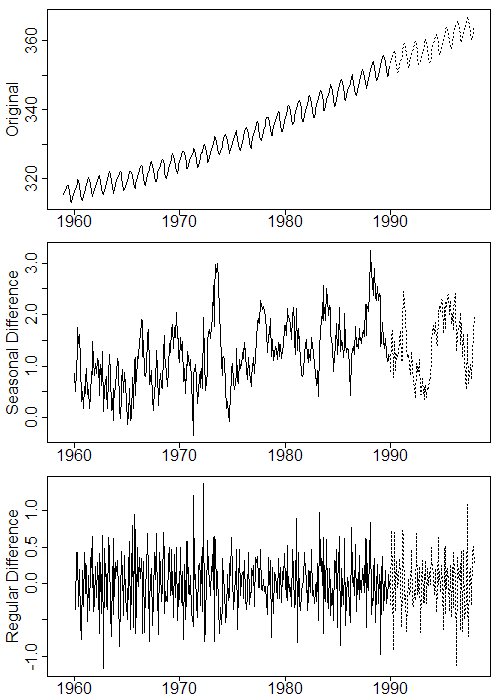
\includegraphics[scale=0.55]{co2plots}
\end{figure}

\begin{figure}[htbp]
	\centering
	\caption{Plots of $x_{2,t}$ (Top),$\Delta_{12}x_{2,t}$ (Middle), and $\Delta_1\Delta_{12}x_{2,t}$ (Bottom) Partitioned Into Fitting (solid) and Forecasting (dotted) Periods}
	\label{fig:co2plots2}
	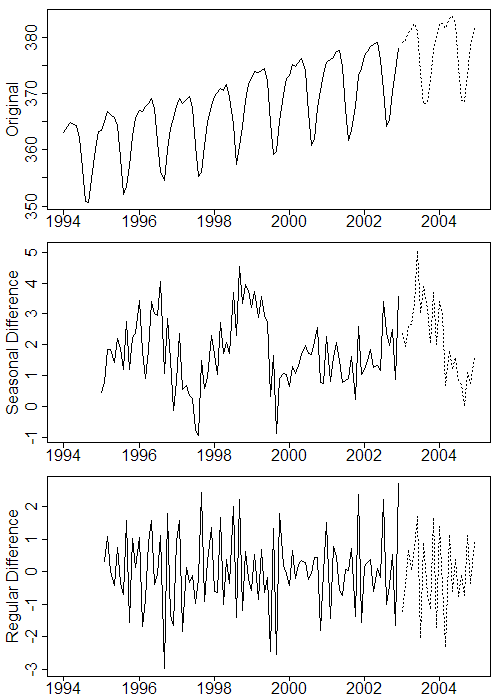
\includegraphics[scale=0.55]{co2plots2}
\end{figure}

The DGPs of $\{y_{1,t}\}$ and $\{y_{2,t}\}$ are hidden to the observer; therefore, evaluating the ability of a subset selection method to uncover the truth is an impossible task. The exploration into various cross-validation methods was motivated by the terminal desire to produce forecasts. Frequentist and Bayesian methods in Tables \ref{tab:aicbic} and \ref{tab:bhstypes} are applied to estimate subset ARMA$(14,14)$ models on the data provided in the fitting period. Methods $\textrm{AL}_5$, $\textrm{AL}_7$, $\textrm{AL}_{10}$ and elastic net counterparts are removed from the consideration because of their similarity to other methods. From the final subset ARMA($14,14$) models, rolling one-step ahead predictions $\hat{y}_{k,t}$ are obtained over the full forecasting period of length $n_k$ where $k\in\{1,2\}$.  As previously determined, $n_1=96$ and $n_2=24$.  

Additionally, three classic methods are explored for baseline forecast performance. First, the naive random walk (RW) model, which does not require estimation, is considered. RW forecasts are obtained via $\hat{y}_{k,t}=y_{k,t-1}$. Next, a saturated ARMA$(\tilde{p},\tilde{q})$ where $\tilde{p}<14$ and $\tilde{q}<14$ is estimated. Finally, a saturated SARMA$(\tilde{p},\tilde{q})\times (\tilde{P},\tilde{Q})_s$, under prior assumptions $s=12$, $\tilde{p}<14$, $\tilde{q}<14$, $\tilde{P}<14$, and $\tilde{Q}<14$, is also used. Best ARMA and SARMA models are selected using {\bf auto.arima()} in the {\bf forecast} package. By default, a stepwise algorithm searches for $\tilde{p}$, $\tilde{q}$, $\tilde{P}$, and $\tilde{Q}$ based on minimization of AIC.

Methods are evaluated based on root mean squared error ($RMSE$), mean absolute scaled error ($MASE$), mean bias ($MB$), and mean directional bias ($MDB$). The formulas for these metrics are expressed in Equation \ref{eq:fmetrics}. $MASE$ is based on errors scaled by the mean absolute error under the naive RW model for the training period ($MAE_{k,\textrm{RW}}$). $MASE<1$ occurs when a method outperforms the naive RW, on average \citep{Hyndman2006}.   In the expression for $MDB$,  $\textrm{sgn}(x_t)=1$ if $x_t>0$ and $\textrm{sgn}(x_t)=-1$ if $x_t<0$. Large values of $RMSE$ and $MASE$ indicate poor predictive accuracy. The bias metrics, $MB$ and $MDB$, are negative when models overestimate future values and positive when models underestimate future values.
\begin{equation}
\label{eq:fmetrics}
\begin{split}
	RMSE_k&=\frac{1}{n_k} \sum\limits_{j=1}^{n_k} (y_{k,j}-\hat{y}_{k,j})^2 \\
	MASE_k&=\frac{1}{n_k} \sum\limits_{j=1}^{n_k} \Bigg|\frac{y_{k,j}-\hat{y}_{k,j}}{MAE_{k,\textrm{RW}}}\Bigg| \\
	MB_k&=\frac{1}{n_k} \sum\limits_{j=1}^{n_k} (y_{k,j}-\hat{y}_{k,j}) \\
	MDB_k&=\frac{1}{n_k} \sum\limits_{j=1}^{n_k} \textrm{sgn}(y_{k,j}-\hat{y}_{k,j})\\
\end{split}
\end{equation}


Starting with the Mauna Loa series $\{y_{1,t}\}$, final subset ARMA$(14,14)$ model selection is summarized in Figure \ref{fig:maunaloaselect}. AR parameters $\{\phi_1,\phi_3,\phi_9\}$ and MA parameters $\{\theta_1,\theta_{12}\}$ are consistently selected. Stationary and invertibility characteristics of ARMA are tested according to the characteristic polynomials. Final models under $\textrm{AL}_4$ and $\textrm{AE}_4$ fail the invertibility assumption, leading to unbounded forecasts. Biasing final model selection on a single OOS period seems to be less protective against non-stationary and non-invertible estimates.  One-step ahead forecast evaluation for the remaining models is displayed in Table \ref{tab:maunaloaselect}. Bayesian methods outperform ADLASSO and ADENET according to all metrics. Forecasts from $\textrm{BHS}_m$ and $\textrm{BHS}^+_m$ for $m\in\{1,2,3,4\}$ are slightly more accurate ($RMSE$ \& $MASE$) and significantly less biased ($MB$ \& $MDB$). 

Forecasting performance from all subset ARMA models is superior to results from the naive RW. Although the bias is relatively low for RW, the error associated with point forecasts is at least double the error for $\textrm{BHS}$ and $\textrm{BHS}^+$. Based on AIC, saturated ARMA$(0,1)$ and SARMA$(0,0,1)$ are selected. The Bayesian subset ARMA models outperform ARMA$(0,1)$. When compared to ADLASSO and ADENET, forecasting accuracy is similar, but $MB$ and $MDB$ show ARMA$(0,1)$ forecasts are less biased. Furthermore, the sign difference in $MDB$ indicates ARMA$(0,1)$ forecasts are occasionally underestimated while $\textrm{AL}$ and $\textrm{AE}$ often overestimate. The SARMA model is extremely competitive to $\textrm{BHS}$ and $\textrm{BHS}^+$. Recall that estimation of SARMA requires knowing the seasonal periodicity $s=12$; and although this is a reasonable assumption, subset ARMA methods do not require this prior belief.

\begin{figure}[htbp]
	\caption{Final Model Selection for Mauna Loa $\textrm{CO}_2$ }
	\center
	\label{fig:maunaloaselect}
	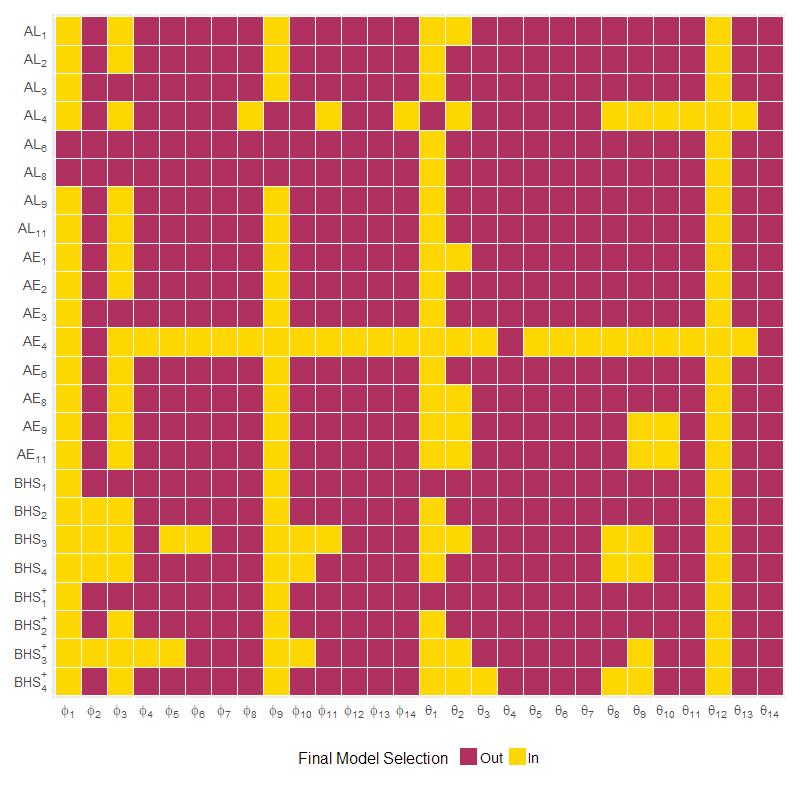
\includegraphics[scale=0.42]{maunaloaselect}
\end{figure}

\begin{table}[htbp]
\footnotesize
\centering
\caption{One-Step Ahead Forecasting Results for Mauna Loa $\textrm{CO}_2$}
\begin{tabular}{c|cc|cc|cc|cc}
  \hline
   & \multicolumn{2}{c|}{$RMSE$} & \multicolumn{2}{c|}{$MASE$} &
  \multicolumn{2}{c|}{$MB$} & \multicolumn{2}{c}{$MDB$}\\
   m & $\textrm{AL}_m$ & $\textrm{AE}_m$ &
  $\textrm{AL}_m$ & $\textrm{AE}_m$ &
  $\textrm{AL}_m$ & $\textrm{AE}_m$ &
  $\textrm{AL}_m$ & $\textrm{AE}_m$ \\
  \hline
  1 & 0.34 & 0.34 & 0.53 & 0.53 & -0.13 & -0.13 & -0.31 & -0.29 \\ 
  2 & 0.33 & 0.33 & 0.52 & 0.52 & -0.10 & -0.10 & -0.21 & -0.21 \\ 
  3 & 0.34 & 0.34 & 0.52 & 0.52 & -0.10 & -0.10 & -0.21 & -0.21 \\ 
  4 & \multicolumn{8}{c}{Not Invertible (NI)} \\ 
  6 & 0.34 & 0.33 & 0.53 & 0.52 & -0.10 & -0.09 & -0.17 & -0.23 \\ 
  8 & 0.34 & 0.34 & 0.53 & 0.54 & -0.10 & -0.14 & -0.19 & -0.31 \\ 
  9 & 0.34 & 0.36 & 0.52 & 0.57 & -0.10 & -0.18 & -0.23 & -0.44 \\ 
  11 & 0.33 & 0.36 & 0.52 & 0.56 & -0.10 & -0.17 & -0.21 & -0.44 \\ 
  \hline
  \hline
     & \multicolumn{2}{c|}{$RMSE$} & \multicolumn{2}{c|}{$MASE$} &
  \multicolumn{2}{c|}{$MB$} & \multicolumn{2}{c}{$MDB$}\\
  m & $\textrm{BHS}_m$ & $\textrm{BHS}^+_m$ &
  $\textrm{BHS}_m$ & $\textrm{BHS}^+_m$ &
  $\textrm{BHS}_m$ & $\textrm{BHS}^+_m$ &
  $\textrm{BHS}_m$ & $\textrm{BHS}^+_m$ \\
  \hline
  1 & 0.31 & 0.31 & 0.49 & 0.49 & -0.01 & -0.01 & 0.04 & 0.06 \\ 
  2 & 0.32 & 0.32 & 0.50 & 0.50 & -0.02 & -0.02 & 0.00 & -0.02 \\ 
  3 & 0.32 & 0.32 & 0.51 & 0.51 & -0.02 & -0.02 & 0.00 & 0.00 \\ 
  4 & 0.32 & 0.32 & 0.50 & 0.50 & -0.01 & -0.01 & 0.02 & 0.02 \\ 
  \hline
  \hline
  m & \multicolumn{2}{c|}{$RMSE$} & \multicolumn{2}{c|}{$MASE$} &
  \multicolumn{2}{c|}{$MB$} & \multicolumn{2}{c}{$MDB$}\\
  \hline
  RW &  \multicolumn{2}{c|}{0.64} & \multicolumn{2}{c|}{1.03} &
  \multicolumn{2}{c|}{0.00} & \multicolumn{2}{c}{-0.02}\\
    ARMA &  \multicolumn{2}{c|}{0.37} & \multicolumn{2}{c|}{0.60} &
  \multicolumn{2}{c|}{0.01} & \multicolumn{2}{c}{0.13}\\
    SARMA &  \multicolumn{2}{c|}{0.30} & \multicolumn{2}{c|}{0.49} &
  \multicolumn{2}{c|}{-0.04} & \multicolumn{2}{c}{-0.02}\\
   \hline
\end{tabular}
\label{tab:maunaloaselect}
\end{table}

In regards to the Alert series $\{y_{2,t}\}$, final subset ARMA$(14,14)$ model selection is summarized in Figure \ref{fig:alertselect}. \citet{Cryer2008} and \citet{Chen2011}  build models for $\{y_{2,t}\}$ but neither evaluate forecasting; therefore, they use the full series for model selection and estimation. Despite this difference, the best subset ARMA model from ADLASSO, containing $\{\phi_1,\phi_{12},\theta_9,\theta_{11},\theta_{12}\}$ , overlaps with many of the final subset ARMA models \citep{Chen2011}. Post ADLASSO, \cite{Chen2011} refit subset SARMA$(1,9)\times(1,1)_{12}$, where both $\phi_1$ and $\phi_{12}$ are deselected. Parameters $\phi_1$ and $\theta_{12}$ are consistently relevant. Recall the similar pattern exhibited for Mauna Loa (Figure \ref{fig:maunaloaselect}). Specifically for Bayesian methods, the seasonal AR parameter $\phi_{12}$ is selected in all final models. For the shorter Alert data, the final AL/AD are more parsimonious than final BHS/$\textrm{BHS}^+$. This effect is not as pronounced for Mauna Loa. This implies that the forecasting advantages from  BHS/$\textrm{BHS}^+$ (see Table \ref{tab:maunaloaselect}) are solely based on the improved estimation of relevant ARMA parameters under Bayesian horseshoe regularization.

Table \ref{tab:alertselect} summarizes one-step ahead forecasting for $\{y_{2,t}\}$. Again, stationarity and invertiblity are checked. Results for $\textrm{AL}_1$, $\textrm{AE}_1$, and $\textrm{AE}_9$ are unreported for failing the invertibility condition. Again, the naive RW produces the worst forecasts. For Alert, saturated ARMA$(1,1)$ and SARMA$(0,1)\times(0,1)_{12}$ are selected. The latter is identical to the one selected in \cite{Cryer2008}. All subset ARMA methods perform as well or better than baseline ARMA, but outperforming the best SARMA  is difficult. In this scenario, there is not a clear divide between the frequentist and Bayesian methods. All results are based on a short time period $(n_2=24)$ and no subset ARMA procedure is definitively superior. 

\begin{figure}[htbp]
	\caption{Final Model Selection for Alert $\textrm{CO}_2$ }
	\center
	\label{fig:alertselect}
	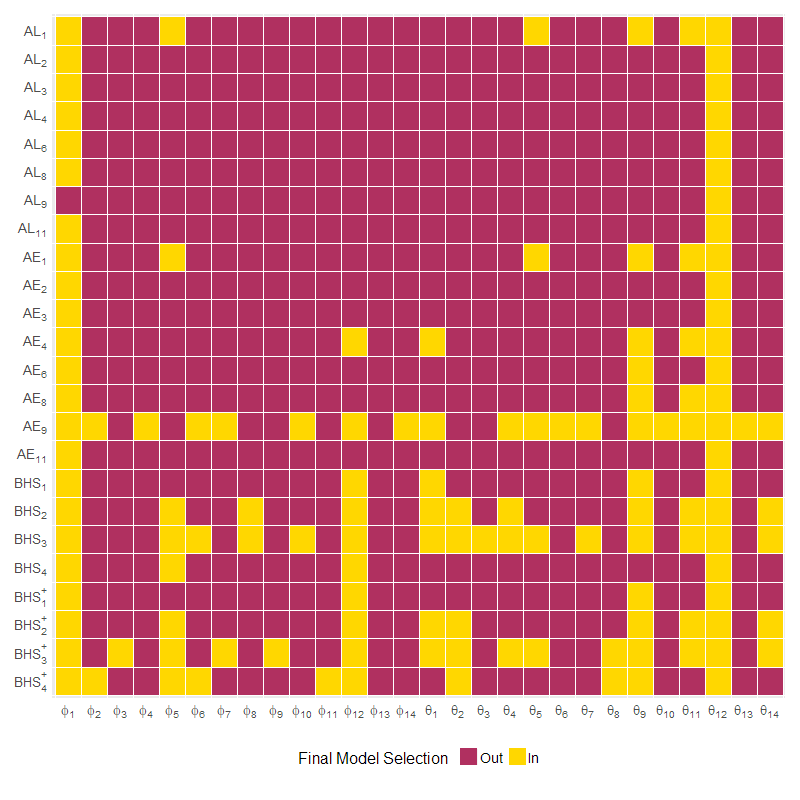
\includegraphics[scale=0.42]{alertselect}
\end{figure}

\begin{table}[ht!]
\footnotesize
\centering
\caption{One-Step Ahead Forecasting Results for Alert $\textrm{CO}_2$}
\begin{tabular}{c|cc|cc|cc|cc}
  \hline
   & \multicolumn{2}{c|}{$RMSE$} & \multicolumn{2}{c|}{$MASE$} &
  \multicolumn{2}{c|}{$MB$} & \multicolumn{2}{c}{$MDB$}\\
   m & $\textrm{AL}_m$ & $\textrm{AE}_m$ &
  $\textrm{AL}_m$ & $\textrm{AE}_m$ &
  $\textrm{AL}_m$ & $\textrm{AE}_m$ &
  $\textrm{AL}_m$ & $\textrm{AE}_m$ \\
  \hline
  1 & \multicolumn{8}{c}{Not Invertible (NI)} \\ 
  2 & 0.84 & 0.84 & 0.43 & 0.43 & 0.03 & 0.03 & 0.08 & 0.08 \\ 
  3 & 0.84 & 0.84 & 0.43 & 0.43 & 0.05 & 0.05 & 0.08 & 0.08 \\ 
  4 & 0.85 & 0.81 & 0.42 & 0.39 & 0.03 & 0.06 & 0.08 & 0.17 \\ 
  6 & 0.86 & 0.81 & 0.41 & 0.42 & -0.07 & 0.12 & 0.08 & 0.33 \\ 
  8 & 0.86 & 0.82 & 0.41 & 0.40 & -0.07 & 0.08 & 0.08 & 0.25 \\ 
  9 & 1.14 & NI & 0.62 & NI & -0.12 & NI & -0.17 & NI \\ 
  11 & 0.86 & 0.84 & 0.41 & 0.41 & -0.07 & -0.02 & 0.08 & 0.08 \\ 
    \hline
  \hline
     & \multicolumn{2}{c|}{$RMSE$} & \multicolumn{2}{c|}{$MASE$} &
  \multicolumn{2}{c|}{$MB$} & \multicolumn{2}{c}{$MDB$}\\
  m & $\textrm{BHS}_m$ & $\textrm{BHS}^+_m$ &
  $\textrm{BHS}_m$ & $\textrm{BHS}^+_m$ &
  $\textrm{BHS}_m$ & $\textrm{BHS}^+_m$ &
  $\textrm{BHS}_m$ & $\textrm{BHS}^+_m$ \\
  \hline
  1 & 0.82 & 0.83 & 0.39 & 0.40 & -0.10 & -0.10 & 0.00 & 0.00 \\ 
  2 & 0.82 & 0.83 & 0.39 & 0.39 & -0.11 & -0.11 & -0.08 & -0.08 \\ 
  3 & 0.81 & 0.82 & 0.38 & 0.39 & -0.11 & -0.11 & -0.08 & -0.08 \\ 
  4 & 0.88 & 0.89 & 0.43 & 0.43 & -0.12 & -0.12 & -0.08 & 0.00 \\ 
  \hline
  \hline
      m & \multicolumn{2}{c|}{$RMSE$} & \multicolumn{2}{c|}{$MASE$} &
  \multicolumn{2}{c|}{$MB$} & \multicolumn{2}{c}{$MDB$}\\
  \hline
    RW &  \multicolumn{2}{c|}{2.11} & \multicolumn{2}{c|}{1.15} &
  \multicolumn{2}{c|}{-0.08} & \multicolumn{2}{c}{0.00}\\
      ARMA &  \multicolumn{2}{c|}{0.91} & \multicolumn{2}{c|}{0.44} &
  \multicolumn{2}{c|}{-0.11} & \multicolumn{2}{c}{0.08}\\
    SARMA &  \multicolumn{2}{c|}{0.79} & \multicolumn{2}{c|}{0.41} &
  \multicolumn{2}{c|}{0.01} & \multicolumn{2}{c}{0.08}\\
   \hline
\end{tabular}
\label{tab:alertselect}
\end{table}

Although a ``best" procedure does not emerge for the Alert series, this example is an opportunity to reemphasize the importance of the stationarity and invertibility conditions. Methods $\textrm{AL}_1$ and $\textrm{AE}_1$  use AIC in the selection of optimal tuning parameters $\lambda^*$ and $\alpha^*$. Each resulting estimate, $\hat{\bm{\beta}}_{AL}(\lambda^*)$ and $\hat{\bm{\beta}}_{AE}(\lambda^*,\alpha^*)$, produce a set of MA coefficients $\hat{\bm{\theta}}$ that represent a non-invertible ARMA process. Naturally, out-of-sample forecasting from $\textrm{AL}_1$ and $\textrm{AE}_1$ is poor and unreported in Table \ref{tab:alertselect}. Both of these approaches for subset ARMA estimation were introduced and demonstrated in \cite{Chen2011}; however, this issue is also present in $\textrm{AL}_4$ and $\textrm{AE}_4$ for Mauna Loa and in $\textrm{AE}_9$ for Alert. Specifically for $\textrm{AL}_1$ and $\textrm{AE}_1$, the grid search across $\mathcal{L}$ and $\mathcal{A}$ is adjusted to only produce estimates of stationary and invertible ARMA process. The final models under $\textrm{AL}_1$ and $\textrm{AE}_1$ identify a new set of relevant parameters $\{\phi_1,\theta_9,\theta_{11},\theta_{12}\}$ which is even closer to the best model identified in \cite{Chen2011}. The adjusted forecasting results from $\textrm{AL}_1$ and $\textrm{AE}_1$ are displayed in Table \ref{tab:alertselect2}. These issues stem from the treatment of ARMA as an unconstrained linear regression, and this approach is inappropriate for nonstationary data. For data that seems to be stationary, i.e. $\{y_{1,t}\}$ and $\{y_{2,t}\}$, ADLASSO and ADENET methods are easily modified to ignore parts of the solution path that violate the important regulatory assumptions. Similarly, BHS and $\textrm{BHS}^+$ can be modified to ignore posterior samples $\bm{\beta}^{(s)}$ and $\sigma^{(s)}$ if $\bm{\beta}^{(s)}$ is not ARMA.

\begin{table}[htbp]
\footnotesize
\centering
\caption{Adjusted One-Step Ahead Forecasting Results for Alert $\textrm{CO}_2$}
\begin{tabular}{c|cc|cc|cc|cc}
  \hline
   & \multicolumn{2}{c|}{$RMSE$} & \multicolumn{2}{c|}{$MASE$} &
  \multicolumn{2}{c|}{$MB$} & \multicolumn{2}{c}{$MDB$}\\
   m & $\textrm{AL}_m$ & $\textrm{AE}_m$ &
  $\textrm{AL}_m$ & $\textrm{AE}_m$ &
  $\textrm{AL}_m$ & $\textrm{AE}_m$ &
  $\textrm{AL}_m$ & $\textrm{AE}_m$ \\
  \hline
  1 & 0.81 & 0.81 & 0.40 & 0.40 & 0.08 & 0.08 & 0.25 & 0.25 \\ 
  \hline
\end{tabular}
\label{tab:alertselect2}
\end{table}



\section{Conclusion}

Subset ARMA$(p,q)$ models are widely applicable for modeling temporal dynamics and forecasting of weakly stationary time series. ARMA modeling via linear regression has advantages and disadvantages. If $p$ and $q$ are intentionally overestimated, frequentist and Bayesian regularization techniques, that shrink irrelevant parameters to $0$ without overshrinking relevant parameters, are easily applied. All regularization methods presented were chosen based on their theoretical oracle properties and capability of handling correlated predictors. However, it is not guaranteed the final $\hat{\bm{\beta}}$ represents a stationary and invertible ARMA process. Simple adjustments to all methods are discussed to remove this problem. Another issue is the sensitivity to the selection of proxy innovations $\{\hat{\epsilon}_t\}$ using a long AR$(p')$ model. It is strongly suggested that initial model selection is not performed for selection of $p'$ at this step.

When ADLASSO or ADENET methods are used to automate estimation and model selection, the approach taken to search for tuning parameters is important. Empirical analysis demonstrates that the true DGP limits the effectiveness of these approaches. Modified BCV-K based on the maximum temporal dependency does not improve model selection or forecasting over CV-K in ADLASSO. Based on simulation results, CV-K is recommended for ADENET regularization. \cite{Bergmeir2018} shows that regular CV-K always outperforms OOS and adequately estimates PE if the considered model is not far from the truth. Although the saturated model is grossly overfitted, estimation via regularization shrinks $\hat{\bm{\beta}}$ to the ``truth," preventing this from being an issue. 

Bayesian regularization via horseshoe priors reduces irrelevant effects but does not perform model selection.  Posterior distributions of subset ARMA$(p,q)$ models can be obtained through projection removing the need for repeated Gibbs sampling. Whether BHS or $\textrm{BHS}^+$ is chosen, a general improvement in model selection and forecasting is observed compared to ADLASSO and ADENET. Also, posterior means $\hat{\bm{\beta}}$ across replications and practicle examples consistently validated stationary and invertible conditions.  However, when the unknown DGP was a subset MA$(q)$ process, BHS and $\textrm{BHS}^+$ rarely selected the corrected model. Combining CV algorithms with BHS and $\textrm{BHS}^+$ may produce better results but are computationally expensive \citep{Peltola2014}; therefore, this is left for future research.

All discussed methods are quick and easy to employ. In Appendix \ref{appendix2}, detailed {\bf R} code is provided to encourage reproducibility. Furthermore, the application of these methods to the Mauna Loa $\textrm{CO}_2$ time series is included to demonstrate usage and illustrate forecasting. 

